\documentclass[12pt,a4paper]{article}
\usepackage[utf8]{inputenc}
%referencing >>>>>>>>
\usepackage{amsmath}
\usepackage{csquotes}% Recommended
\usepackage[english]{babel}
\usepackage[maxbibnames=99, giveninits=true, sorting=none,style=authoryear-ibid,backend=biber,doi=false,isbn=false,eprint=false]{biblatex}
\addbibresource{bibliography.bib}% Syntax for version >= 1.2
%for minted>>>>>
\usepackage{minted}
\usemintedstyle{colorful}
%others >>>>>>>>
\usepackage{amsmath}
\usepackage{graphicx}
\usepackage{float}
\usepackage[center]{caption}
\usepackage[normalem]{ulem}
\usepackage{longtable}
\usepackage{comment}
\usepackage{array}
\usepackage{soul}
\usepackage{fancyhdr}
\usepackage{adjustbox}
\usepackage{amsmath}
\usepackage{amssymb}
\usepackage{zed-csp}
\usepackage{geometry}
\usepackage{listings}
\usepackage{xcolor}
\usepackage{titlesec}
%for links >>>>>>
\usepackage{hyperref}

\setcounter{secnumdepth}{4}
\titleformat{\paragraph}
{\normalfont\normalsize\bfseries}{\theparagraph}{1em}{}
\titlespacing*{\paragraph}
{0pt}{3.25ex plus 1ex minus .2ex}{1.5ex plus .2ex}

\titleclass{\subsubsubsection}{straight}[\subsection]

\newcounter{subsubsubsection}[subsubsection]
\renewcommand\thesubsubsubsection{\thesubsubsection.\arabic{subsubsubsection}}
\renewcommand\theparagraph{\thesubsubsubsection.\arabic{paragraph}} % optional; useful if paragraphs are to be numbered
\hypersetup{
    colorlinks=true,
    linkcolor=black,     
    urlcolor=blue,
    citecolor = black
}

\titleformat{\subsubsubsection}
  {\normalfont\normalsize\bfseries}{\thesubsubsubsection}{1em}{}
\titlespacing*{\subsubsubsection}
{0pt}{3.25ex plus 1ex minus .2ex}{1.5ex plus .2ex}

\makeatletter
\renewcommand\paragraph{\@startsection{paragraph}{5}{\z@}%
  {3.25ex \@plus1ex \@minus.2ex}%
  {-1em}%
  {\normalfont\normalsize\bfseries}}
\renewcommand\subparagraph{\@startsection{subparagraph}{6}{\parindent}%
  {3.25ex \@plus1ex \@minus .2ex}%
  {-1em}%
  {\normalfont\normalsize\bfseries}}
\def\toclevel@subsubsubsection{4}
\def\toclevel@paragraph{5}
\def\toclevel@paragraph{6}
\def\l@subsubsubsection{\@dottedtocline{4}{7em}{4em}}
\def\l@paragraph{\@dottedtocline{5}{10em}{5em}}
\def\l@subparagraph{\@dottedtocline{6}{14em}{6em}}
\makeatother


%New colors defined below
\definecolor{codegreen}{rgb}{0,0.6,0}
\definecolor{codegray}{rgb}{0.5,0.5,0.5}
\definecolor{codepurple}{rgb}{0.58,0,0.82}
\definecolor{backcolour}{rgb}{0.95,0.95,0.92}

\lstdefinelanguage{JavaScript}{
  keywords={typeof, new, true, false, catch, function, return, null, catch, switch, var, if, in, while, do, else, case, break},
  keywordstyle=\color{blue}\bfseries,
  ndkeywords={class, export, boolean, throw, implements, import, this},
  ndkeywordstyle=\color{darkgray}\bfseries,
  identifierstyle=\color{black},
  sensitive=false,
  comment=[l]{//},
  morecomment=[s]{/*}{*/},
  commentstyle=\color{purple}\ttfamily,
  stringstyle=\color{red}\ttfamily,
  morestring=[b]',
  morestring=[b]"
}

%Code listing style named "mystyle"
\lstdefinestyle{mystyle}{
  backgroundcolor=\color{backcolour}, commentstyle=\color{codegreen},
  keywordstyle=\color{magenta},
  numberstyle=\tiny\color{codegray},
  stringstyle=\color{codepurple},
  basicstyle=\ttfamily\footnotesize,
  breakatwhitespace=false,         
  breaklines=true,                 
  captionpos=b,                    
  keepspaces=true,                 
  numbers=left,                    
  numbersep=5pt,                  
  showspaces=false,                
  showstringspaces=false,
  showtabs=false,                  
  tabsize=2
}
\lstset{style=mystyle}

\PassOptionsToPackage{hyphens}{url}\usepackage{hyperref}
\hypersetup{
    colorlinks=true,
    linkcolor=black,     
    urlcolor=black,
}
\urlstyle{same}

\graphicspath{ {img/} }

\title{NoSQL database with IoT system}
\author{Zan Zver}
\date{15.05.2022}

\newcommand{\latex}{\LaTeX\ }
\newcommand{\authorName}{Zan Zver}
\newcommand{\authorID}{18133498}
\newcommand{\reportTitle}{Report Title}
\newcommand{\degreeAward}{BSc (Hons) in Computer and Data Science } 

\begin{document}
\DeclareGraphicsExtensions{.jpg,.png,.gif,.pdf,.jpeg}
\begin{titlepage}
   \begin{center}
       CMP6207 Modern Data Stores
       \vspace*{0.5cm}

       \huge\textbf{\reportTitle} 

       \vspace{0.5cm}
        Coursework Assignment Report
            
       \vspace{1.5cm}

       \authorName \\
       \authorID\\
       \vspace{0.5cm}
       \large{Word count: 3685}


       \vfill
            
       \vspace{0.8cm}
     
       \begin{figure}[htp]
        \centering
        
\includegraphics{logo}
        \end{figure}
            
       \large{Faculty of Computing, Engineering and the Built Environment \\
       Birmingham City University \\}
            
   \end{center}
\end{titlepage}
\pagestyle{fancy}
\fancyhf{}
\rhead{
\includegraphics[width = 3.3cm]{header.jpg}}
\lhead{\footnotesize BIRMINGHAM CITY UNIVERSITY \\ SCHOOL OF COMPUTING AND DIGITAL TECHNOLOGY}
\rfoot{Page \thepage}
\newgeometry{top=110pt}
\setlength{\headsep}{50pt}

\tableofcontents

\listoftables

\listoffigures

\lstlistoflistings

\newpage

%\begin{abstract}
%    Summary of the entire report
%\end{abstract}

\section{Types of NoSQL databases}

NoSQL stands for not structured SQL. Since there is no structure, a lot of companies have created NoSQL management system in different ways. All of them are trying to achieve the same goal of efficiency and uptime but with different approaches \parencite{web:Hackolade}. Here are some of more well known and used approaches:
\begin{itemize}
  \item NoSQL Document
  \begin{itemize}
      \item basic unit of data is "Document", we would call that Row in SQL,
      \item document is ordered set of key-value pairs,
      \item are schema free,
      \item represented simple structure is: database, collection (or table in SQL), document.
  \end{itemize}
  
  \item NoSQL Columnar
  \begin{itemize}
      \item data is stored with column oriented model,
      \item uses keyspace model which is similar to schema in relational databases,
      \item represented simple structure is: keyspace, column family, rows, columns.
  \end{itemize}
  
  \item NoSQL Property Graph
  \begin{itemize}
      \item organises data in graph represented structure,
      \item is made of nodes (represents an entity) and edges (represents connection/relationships between two nodes).
  \end{itemize}
  
  \item NoSQL Key-Value
  \begin{itemize}
      \item every item is stored as key-value,
      \item data is stored as a collection of key-value pairs,
      \item key must be unique.
  \end{itemize}
  
  \item NoSQL Multi-model
  \begin{itemize}
      \item joins the previous NoSQL types (Document, Graph, Key-Value) together,
      \item instead of using 3 different NoSQL types in a project, 1 multi-model can be used to provide the same functionality.
  \end{itemize}
\end{itemize}

\begin{center}
\begin{longtable}{ |l|l|l| } 
 \hline
 NoSQL type & DB provider & Well known for \\ 
 \hline
 Document & \vtop{\hbox{\strut MongoDB,}\hbox{\strut Couchbase,}\hbox{\strut AmazonDocument DB,}\hbox{\strut etc...}} & \vtop{\hbox{\strut Used in big data companies}\hbox{\strut(example: BCU, Tesco)}} \\ 
 \hline
 Columnar & \vtop{\hbox{\strut Cassandra DataStax,}\hbox{\strut HBase,}\hbox{\strut BigTable,}\hbox{\strut etc...}} & \vtop{\hbox{\strut Used for big/enormous data storage }\hbox{\strut(example: Facebook, Netflix)}} \\ 
 \hline
 Property Graph & \vtop{\hbox{\strut Neo4j,}\hbox{\strut JanusGraph,}\hbox{\strut TigerGraph,}\hbox{\strut etc...}} & Fast relationship queries \\ 
 \hline
 Key-Value & \vtop{\hbox{\strut DynamoDB,}\hbox{\strut Redis,}\hbox{\strut Aerospike,}\hbox{\strut etc...}} & Fast and simply scalable \\ 
 \hline
 Multi-model & \vtop{\hbox{\strut CosmosDB,}\hbox{\strut Marklogic,}\hbox{\strut OrientDB,}\hbox{\strut etc...}} & Combination of NoSQL types \\ 
 \hline

\caption{NoSQL types compared}
\end{longtable}
\end{center}
\newpage

\section{Relational VS NoSQL databases}

\subsection{About Relational databases}
Relational databases use SQL as their query language.
Relational databases (RDBS) have a clear structure. There is DB, then table and data \parencite{web:MSDatabases}. Database is collection of tables and table is collection of data. Schema is enforced, meaning we have strict data types and requirements where data needs to go.

Every table has fields (columns) and records (rows). Every record has the same number of fields unlike NoSQL.

To improve SQL performance, normalisation is performed. With this, one table is broken apart to multiple tables with primary keys and foreign keys \parencite{kohler2018sql}
\newline
Types of relations:
\begin{itemize}
  \item One to one,
  \item many to many,
  \item one to many,
  \item many to one.
\end{itemize}

\subsection{About NOSQL}
Mongo has the structure of: database, collection, documents. Database can have multiple collections and collection can have multiple documents \parencite{web:AboutMongo}. As name suggests, NoSQL means no schema. That means collection can have documents with different sizes inside.
\newline
NoSQL is flexible ${\xrightarrow{}}$ you can add new data to one document and that one document would be different than others\parencite{web:MongoNoSQL}.
\newline
NoSQL does not have relations. They can be implemented (on software level) but they are not enforced with managment system. Due to this, if the data changes, you need to do multiple updates.

\subsection{Cap theorem}
Stands for:
\newline
C - Consistency - data is the same across the database
\newline
A - Availability - as the data is written, it is replicated to other nodes
\newline
P - Partition tolerance - if node goes offline, how can it be replaced
\newline
\parencite{khazaei2016choose}

\begin{figure}[H]
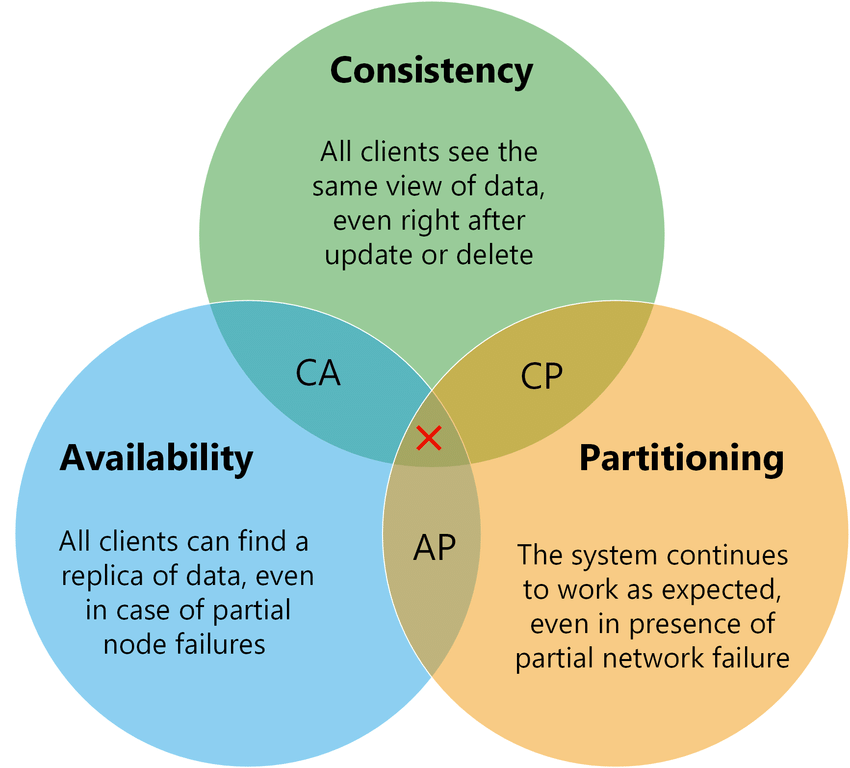
\includegraphics[scale=0.45]{img/CAP.jpeg}
\centering
\caption{CAP theorem representation}
\end{figure}

MongoDB goes under CP, that meaning it is consistent and it has partition tolerance. This is achieved by MongoDB having primary node who receives all the writes and secondary nodes replicate the data after it has been written to primary (consistency). If primary node goes offline, secondary nodes can take over (partition tolerance). MongoDB does not have availability (or HA - high availability) due to it having one master node. So if master node goes offline it takes some time for voting process to be accomplished.

MySQL (relational database) would be CA. Data is written only to one node at the time, this is resulting in consistency. All of the data is also replicated to another node which is resulting in availability. But if master node goes down there is no partitioning in place.

Cassandra on the other hand, is classified as AP. All of the nodes are independent, that is preventing it to have consistency. But due to them not having a master node, read/write can be done from any node and this is resulting in high availability. Nodes are also copying data across to other nodes, this is resulting data (partition) tolerance.
\parencite{web:IBMCAP}

\subsection{Pros for SQL}
\begin{itemize}
  \item uses schemas ${\xrightarrow{}}$ more fixed structure
  \item relations ${\xrightarrow{}}$ no duplicate data, only update once
  \item data is distributed across multiple tables
  \item scaling is vertical
\end{itemize}

\subsection{Pros for NoSQL}
\begin{itemize}
  \item no schema ${\xrightarrow{}}$ data structure can change
  \item relations are not common ${\xrightarrow{}}$ not querying relations 
  \item data is nested in collections together
  \item can scale horizontal and/or vertical
  \item great performance for mass requests
\end{itemize}

\subsection{Scaling}
Scaling can be done in two ways \parencite{cattell2011scalable}
\newline
Horizontal:
\begin{itemize}
    \item add more servers (nodes) and merge data into one DB
    \item data is split across across the servers
\end{itemize}
Vertical:
\begin{itemize}
    \item add more power (upgrade hardware) to existing server 
    \item there is limit of to where you can scale
\end{itemize}



\subsection{Which one is better: SQL or NoSQL}
At the end, it depends on the scenario that we are in. Based on the CAP theorem, lets consider 3 cases:
\begin{itemize}
  \item Consistency and availability (CA)
      \begin{itemize}
        \item This would be for financial institutions, where data needs to be in sync as well as the same.
      \end{itemize}
  \item Consistency and partition tolerance (CP)
      \begin{itemize}
        \item This would be for e-commerce websites where data needs to be consistent and can operate even if node fails. 
      \end{itemize}
  \item Availability and partition tolerance (AP)
      \begin{itemize}
        \item This would be for social media services (like Facebook) where data can be out of sync for some time.
      \end{itemize}
\end{itemize}

Since there is not a clear winner, we can use what is the best for companies use case. Lets use Facebook as an example. They have social media which could be AP, marketplace could be CP and transactions on the site itself which are CA. With this, a company like Facebook can use SQL or NoSQL with correct CAP use case when needed. 
\newline
To have a better representation on how data would be stored in data center, have a look on appendix A1-data centers.
\newpage

\section{IoT NoSQL database}

\subsection{Design}

\subsubsection{Stage 1}
At first stage, we have a look at what our goal is. To explain it from top perspective, we are looking to have a connection to API which is going to access database.
\newline
\begin{figure}[H]
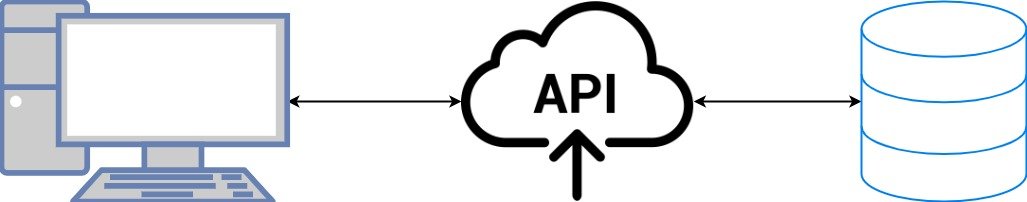
\includegraphics[scale=0.3]{img/systemDiagram-simplev.jpg}
\centering
\caption{Diagram of stage 1}
\end{figure}

\subsubsection{Stage 2}
In the second stage, we define our tools. For database, it is going to be MongoDB. API used for connections is Node with Express (and Mongoose) API. Then we serve the data to the users as NodeJS website or to IoT devices.
\newline
\begin{figure}[H]
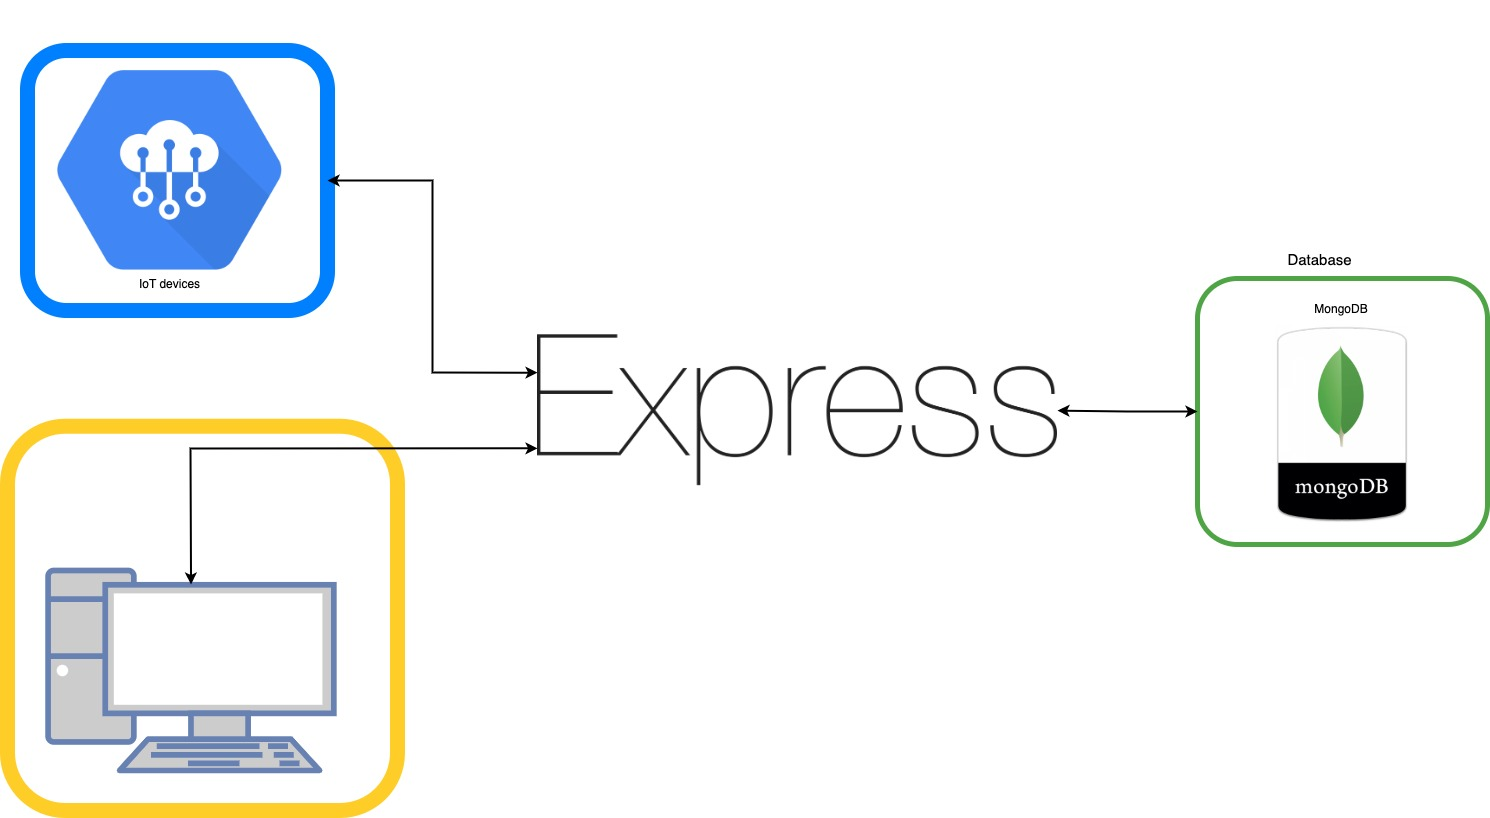
\includegraphics[scale=0.3]{img/systemDiagram-simplev2.jpg}
\centering
\caption{Diagram of stage 2}
\end{figure}

\subsubsection{Stage 3}
Third step defines structure for database and IoT. As seen in the diagram, Docker containers are going to be used for running the database. To improve database up time, we are going to shard it. 
This gives us 5 docker containers:
\begin{itemize}
  \item 1 primary node - all of the writes come to this node
  \item 2 secondary nodes - reads are done from secondary node to balance load off the main node. 
  \item 1 arbiter - in case that primary node goes down, this node is a tiebreaker of election between two of the nodes. This node cannot become primary node.
  \item 1 hidden node - this is backup node. It is hidden, meaning that it cannot participate in election process or in tie breaking. The only duty it has is to copy data from main node to itself. In case there is data loss, this node should have backups.
\end{itemize}
We have also expended on IoT side. Onece connection comes from API, it goes to user or IoT. Our API cannot communicate directly with IoT devices, but it needs some sort of "man in the middle". For that, we would expect API to communicate with the protocols (Apple home kit, Google home, Zigbee, Zwave) and they would comunicate with devices.
\newline
\begin{figure}[H]
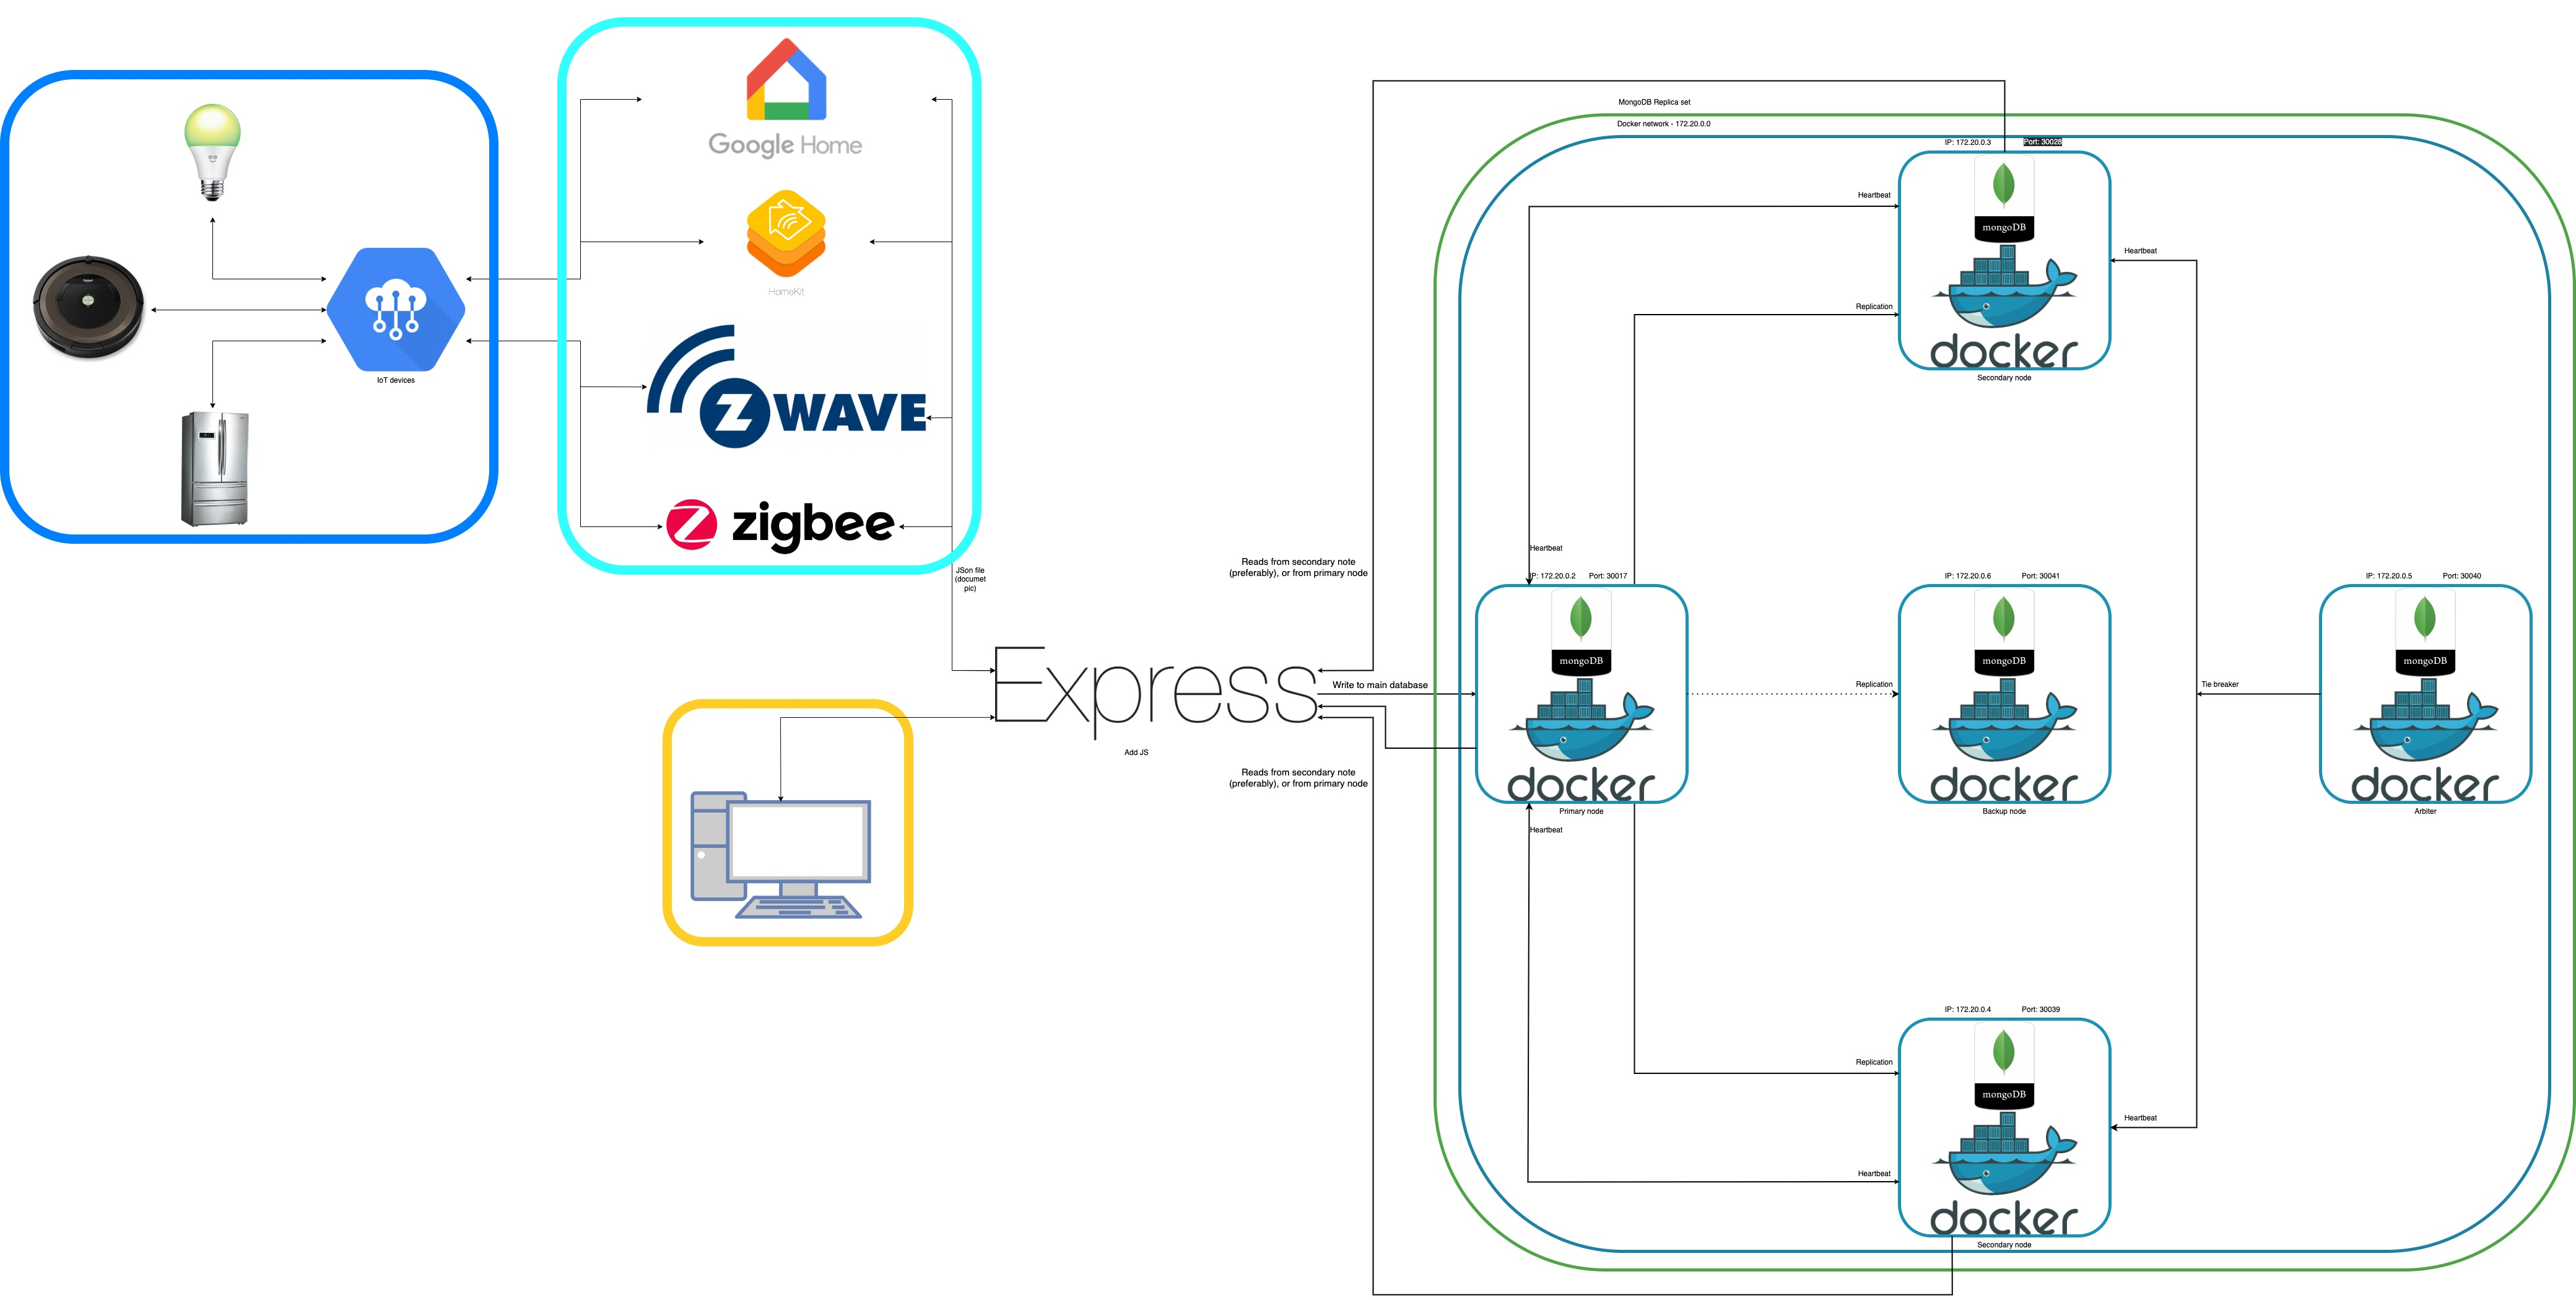
\includegraphics[scale=0.1]{img/systemDiagram-sharded.jpg}
\centering
\caption{Diagram of stage 3}
\end{figure}

\subsubsection{Stage 4}
In stage four, we upgrade our sharded database structure to clustered database structure. With that in mind, shard from step 3 was duplicated to create shard 1-3. With this, two shards can go "offline" and we would still have our data. As seen, we have added 3 new docker containers between API and our cluster. Those are routers. Router is "directing" the traffic between API and shards in our cluster. We have 3 routers in case one of them goes down.
\newline
\begin{figure}[H]
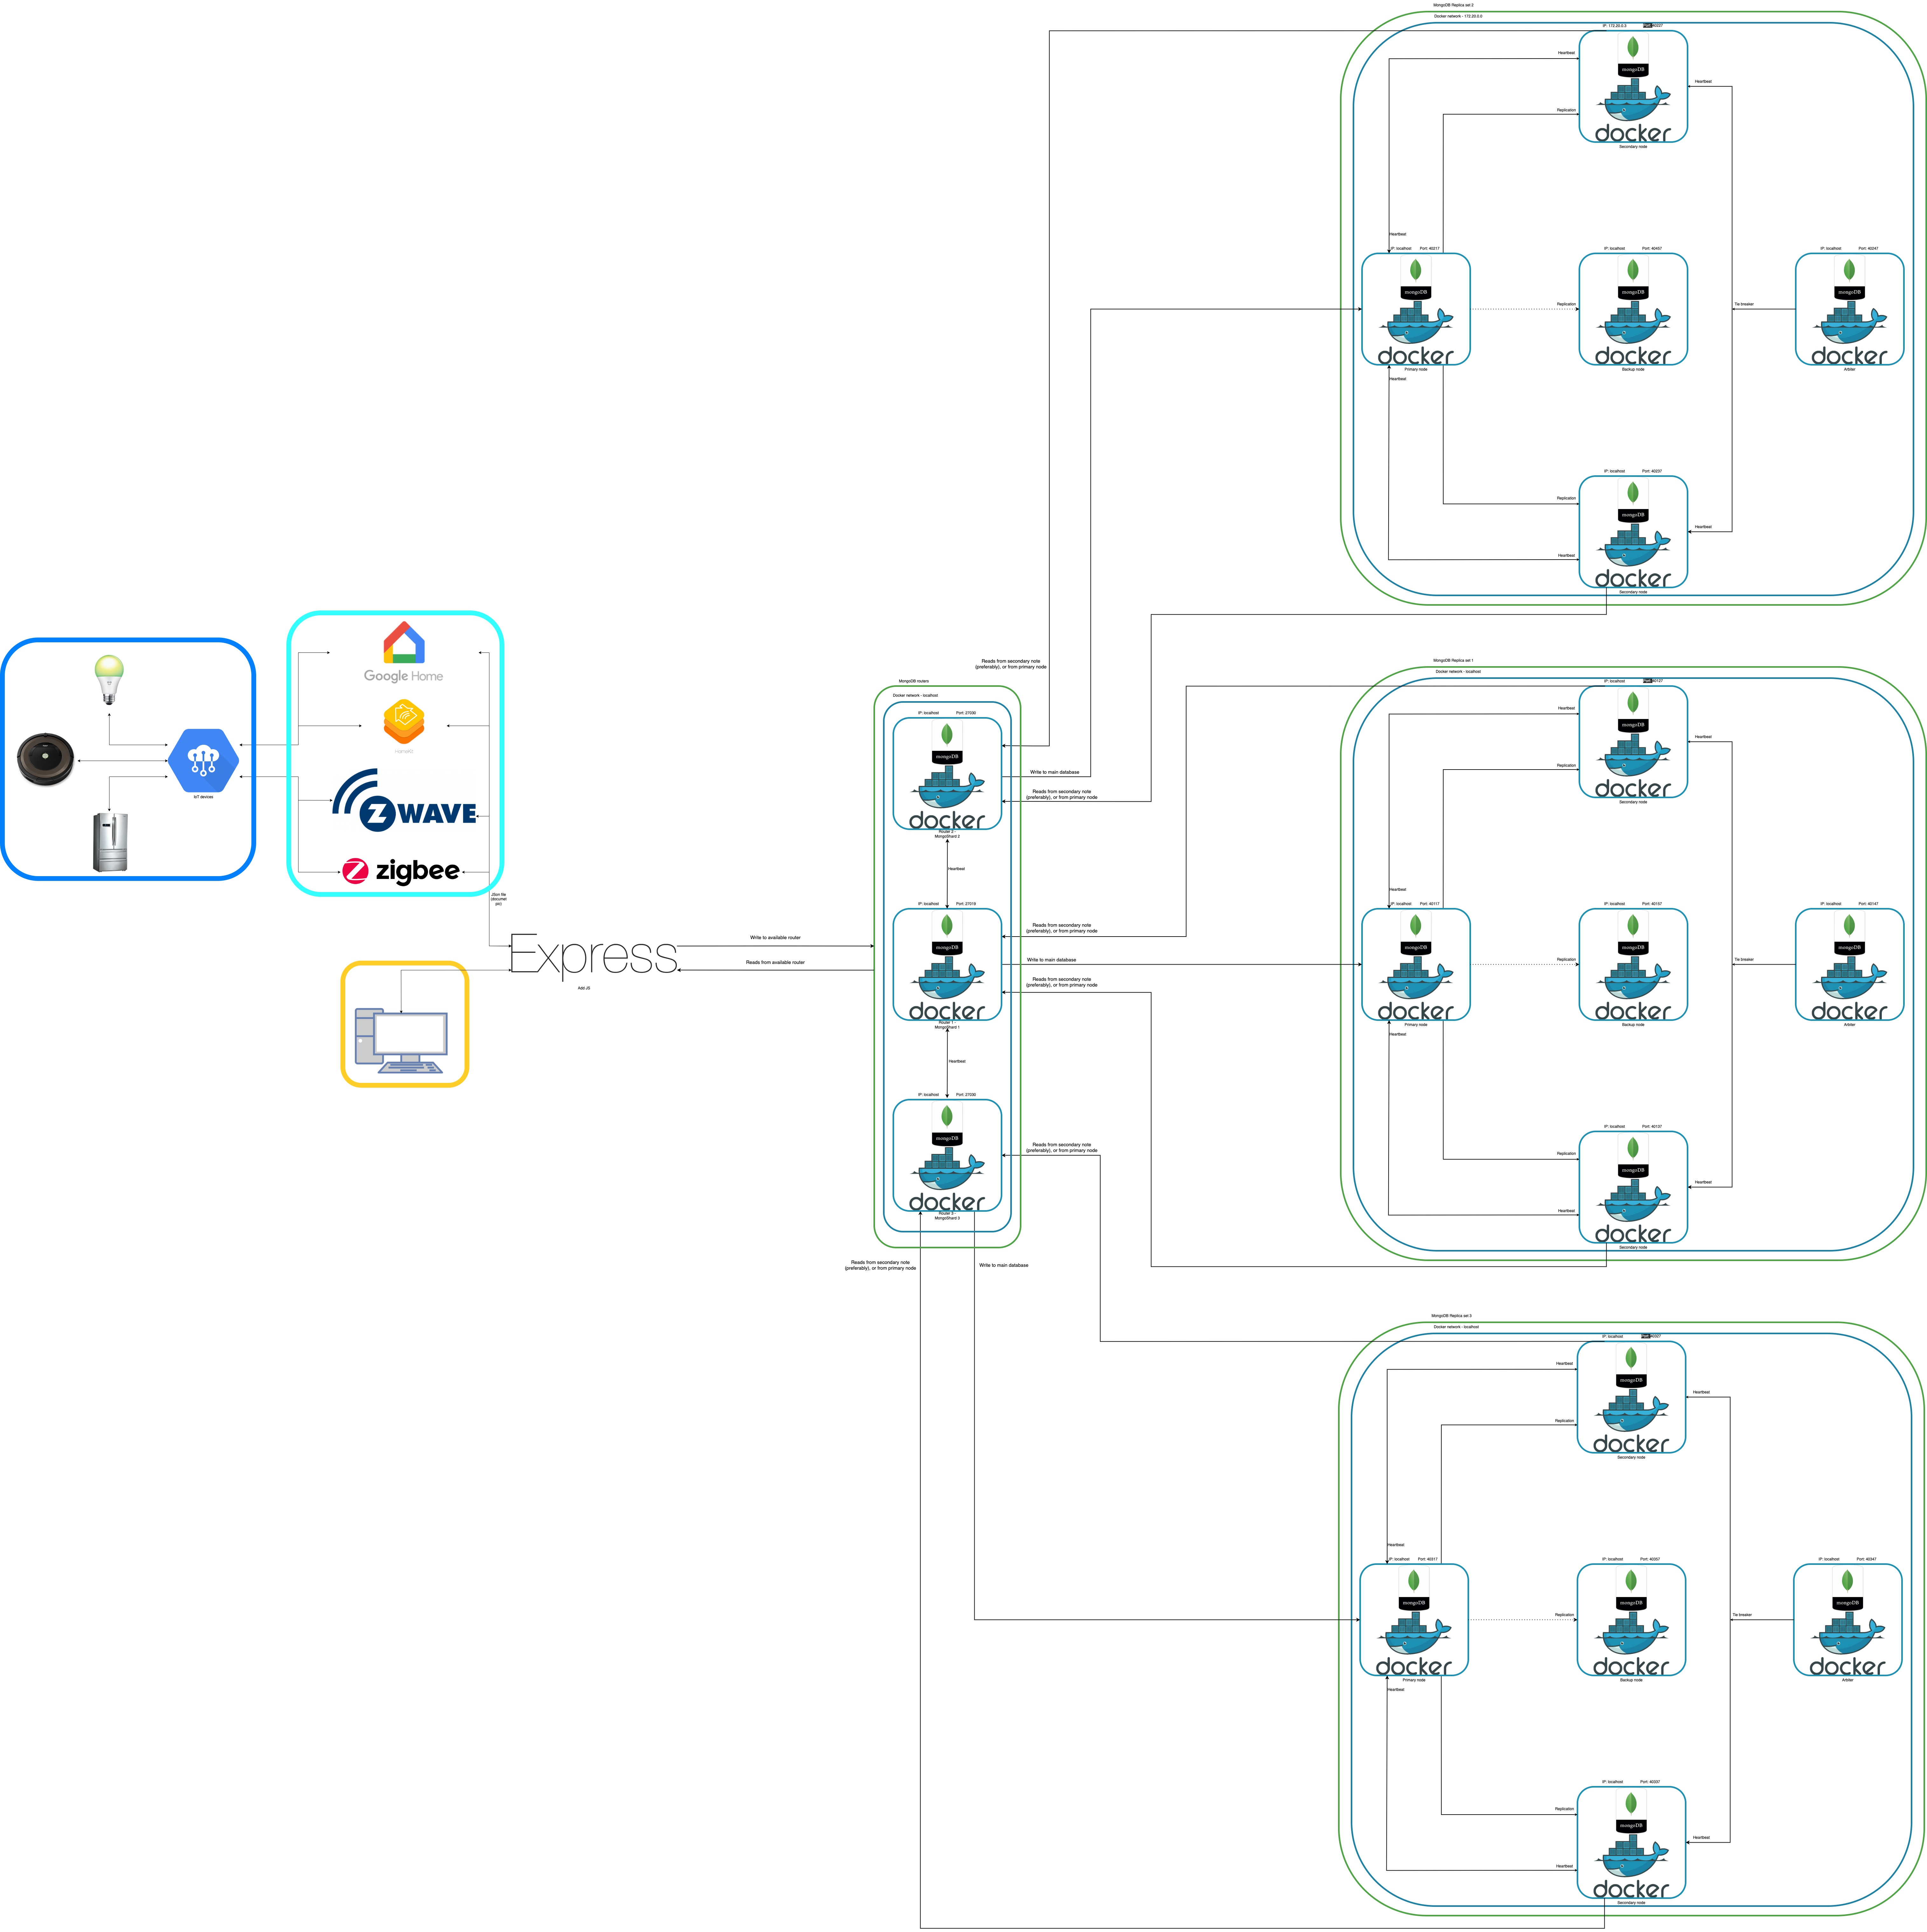
\includegraphics[scale=0.07]{img/systemDiagram-clustered.jpg}
\centering
\caption{Diagram of stage 4}
\end{figure}

\subsubsection{Stage 5}
The final stage is just a concept of security. If we wanted to have all of the connections secured behind the private network (for security reasons), we would put a VPN in front of API. With that, users with VPN credentials can connect to API. Since devices cannot connect directly to VPN (except if network would route directly to VPN), we would configure API to allow reads or writes from the protocols. With that, IoT devices can still communicate with our network but "hackers" cannot get to our API. If we wanted to add extra security, protocols would be set to read only outside of VPN.
\newline
\begin{figure}[H]
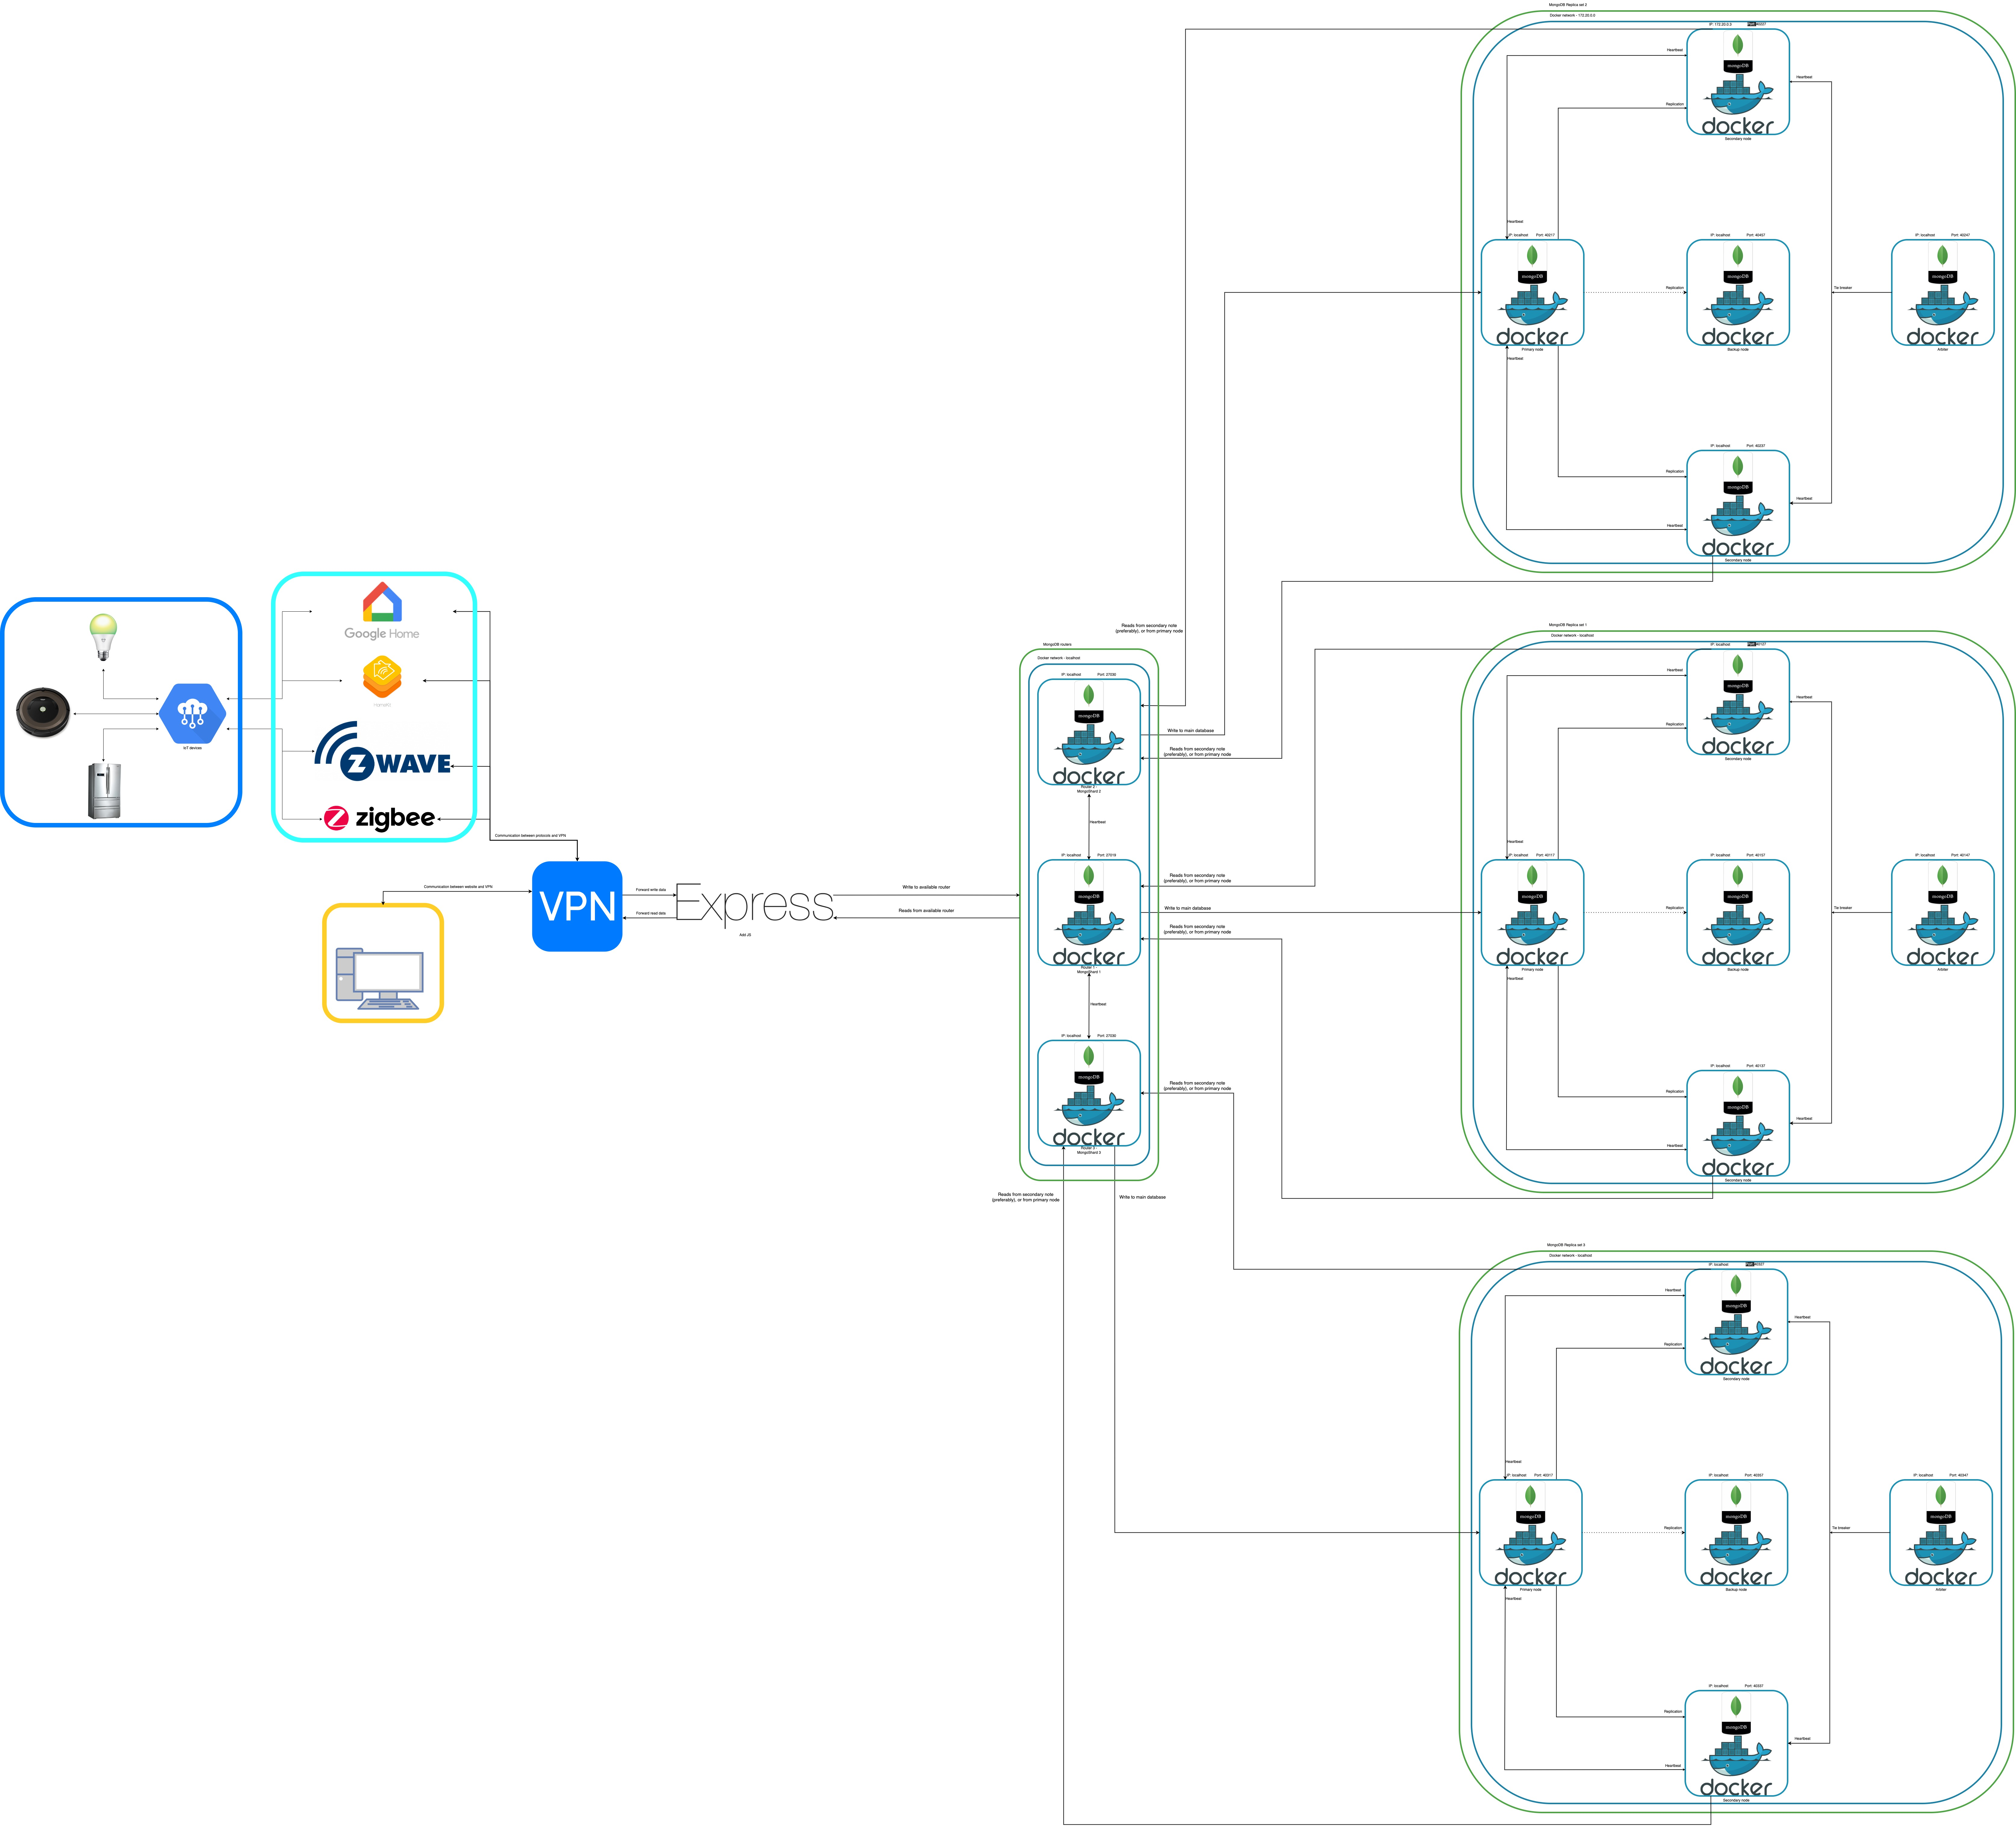
\includegraphics[scale=0.06]{img/systemDiagram-clusteredWithVPN.jpg}
\centering
\caption{Diagram of stage 5}
\end{figure}

As seen from the diagrams above, Docker \parencite{rad2017introduction} is going to be used for hosting the MongoDB \parencite{web:MongoDocker}. Reasons for that are: efficiently, simplicity and scalability.
\begin{center}
\begin{longtable}{ |m{4cm}|m{9cm}| } 
 \hline
 Reasoning & Description \\ 
 \hline
  Efficiently & 
  \begin{itemize}
    \item Docker containers are more light weight in comparison to VMs. This gives them an advantage in terms of OS storage and speed.
  \end{itemize} \\ 
  \hline
  Simplicity & 
  \begin{itemize}
    \item Starting up new docker container is simple. For our use case, we are using Docker Compose. With this, we can have predefined YAML file that has specifications for desired Docker container.
  \end{itemize} \\ 
   \hline
  Scalability & 
  \begin{itemize}
    \item Scaling with MongoDB and Docker is simple. We can scale vertically by adding more docker containers to our network or upgrading existing host server.
  \end{itemize} \\ 
 \hline
\caption{Reasons to use docker}
\end{longtable}
\end{center}


For our IoT database, we are using 4 collections:
\begin{center}
\begin{longtable}{ |m{4cm}|m{9cm}| } 
 \hline
 Collection name & Collection description \\ 
 \hline
  users & 
  \begin{itemize}
    \item has user data inside
    \item read writes from users and admins
  \end{itemize} \\ 
  \hline
  iot{\_}customer{\_}devices & 
  \begin{itemize}
    \item saves customers devices
    \item read writes from users and admins
  \end{itemize} \\ 
   \hline
  iot{\_}device{\_}history & 
  \begin{itemize}
    \item historical list of device status changes
    \item read writes from users and admins
    \item this can be a capped collection, saving changes for a month
  \end{itemize} \\ 
   \hline
  iot{\_}device{\_}info & 
  \begin{itemize}
    \item devices that are supported in the application
    \item users are set to read only, while admins can do read and write
  \end{itemize} \\ 
 \hline
\caption{Collections from DB and their descriptions}
\end{longtable}
\end{center}


\begin{figure}[H]
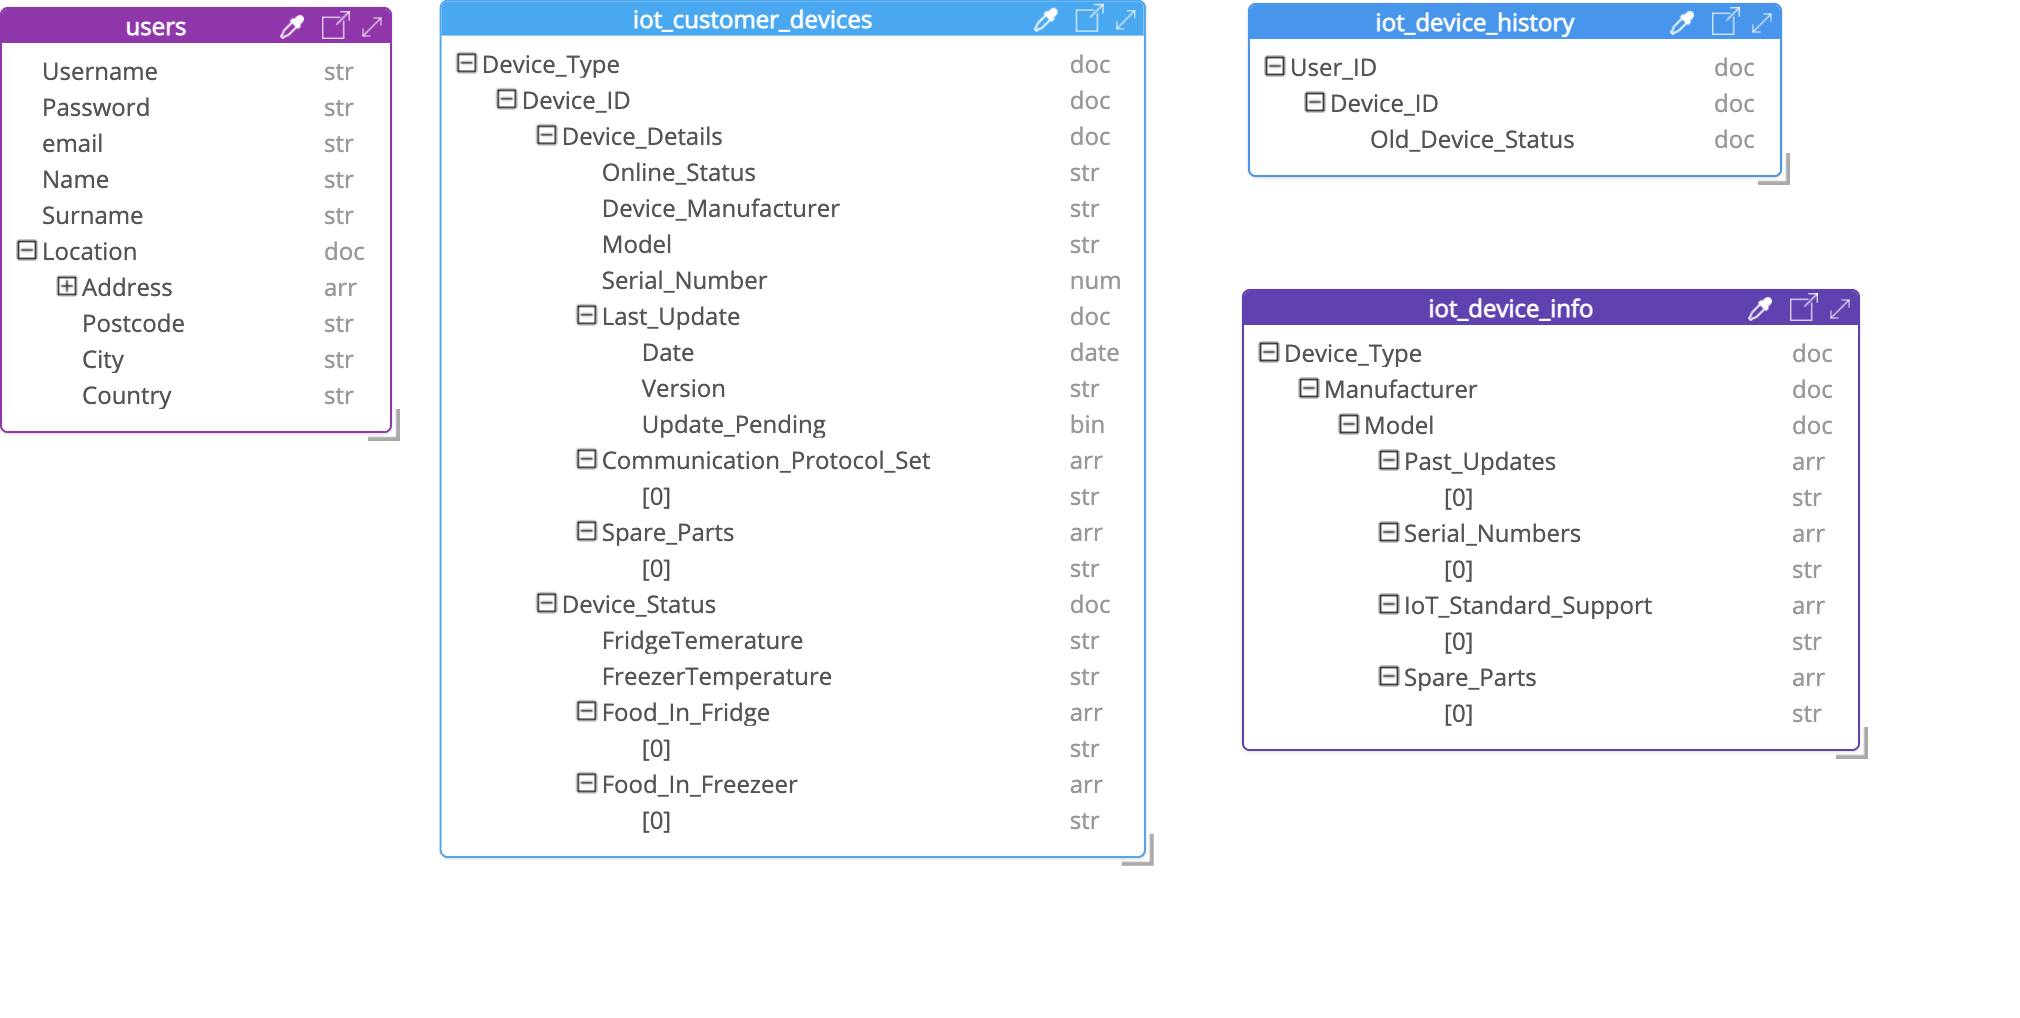
\includegraphics[scale=0.22]{img/IoT_Model_diagram.jpg}
\centering
\caption{Collections diagram}
\end{figure}

users collection document description:
\begin{center}
\begin{longtable}{ |m{4cm}|m{9cm}| } 
 \hline
  Document name & Document description \\ 
 \hline
  Username & 
  \begin{itemize}
    \item Type: string
    \item Must be unique username that would be at least 6 characters long.
  \end{itemize} \\ 
 \hline
  Password &   
  \begin{itemize}
    \item Type: string
    \item User defined password that is at least 8 characters long and it has symbols in. Cannot be the same as username or email.
  \end{itemize} \\
 \hline
  Email &   \begin{itemize}
    \item Type: string
    \item Must be unique and must meet certain expectations (example: have @ in string).
  \end{itemize} \\ 
 \hline
  Name &   \begin{itemize}
    \item Type: String
    \item Name of the user
  \end{itemize} \\
 \hline
  Surname &   
  \begin{itemize}
    \item Type: String
    \item Surname of the user
  \end{itemize} \\ 
 \hline
  Location &   
  \begin{itemize}
    \item Type: document
    \item Is build with 4 other sub items
        \begin{itemize}
            \item Address
                \begin{itemize}
                    \item Type: Array (length of 2)
                    \item Address line 1 is mandatory while address line 2 is optional
                \end{itemize}
            \item Postcode
                \begin{itemize}
                    \item Type: String
                    \item Postcode where user is located
                \end{itemize}
            \item City
                \begin{itemize}
                    \item Type: String
                    \item City where user is located
                \end{itemize}
            \item Country
                \begin{itemize}
                    \item Type: String
                    \item Country where user is located
                \end{itemize}
        \end{itemize}
 \end{itemize} \\
 \hline
\caption{Documents from users collection described}
\end{longtable}
\end{center}

iot{\_}customer{\_}devices collection document description
\begin{center}
\begin{longtable}{ |m{4cm}|m{9cm}| } 
 \hline
 Document name & Document description \\ 
 \hline
  Device{\_}Type &   
  \begin{itemize}
    \item Type: document
    \item Key is device name (example: smart{\_}light) and value is document which has devices inside
  \end{itemize} \\
 \hline
   Device{\_}ID &   
  \begin{itemize}
    \item Type: document
    \item Key is ID of device and value is device{\_}details and device{\_}status
  \end{itemize} \\
 \hline
   Device{\_}Details &   
  \begin{itemize}
    \item Type: document
    \item This document structure is the same across all the devices regardless of their type. Idea of this is to get device meta data which would be the same across the board.
    \begin{itemize}
        \item Online{\_}Status
        \begin{itemize}
            \item Type: boolian
            \item If the device is online or offline.
        \end{itemize}
        
        \item Device{\_}Manufacturer
        \begin{itemize}
            \item Type: String
            \item Who produced the device
        \end{itemize}
        
        \item Model
        \begin{itemize}
            \item Type: String
            \item Model name
        \end{itemize}
        
        \item Serial{\_}Number
        \begin{itemize}
            \item Type: number or String
            \item Serial{\_}number of the device.
        \end{itemize}
        
        \item Last{\_}Update
        \begin{itemize}
            \item Type: document
            \item When was device last updated.
        \end{itemize}
        
        \item Communication{\_}Protocol{\_}Set
        \begin{itemize}
            \item Type: array
            \item Based on available communication protocols, what protocols are being used.
        \end{itemize}
        
        \item Spare{\_}Parts
        \begin{itemize}
            \item Type: array
            \item If there are any spare parts available for purchase, they are listed here.
        \end{itemize}
    \end{itemize} 
  \end{itemize} \\
 \hline
   Device{\_}Status &   
  \begin{itemize}
    \item Type: document
    \item This document depends on device type. In the image above we have an example of what it would look like for smart fridge. But the idea is that device{\_}status gathers data that is from hardware level (example: battery level or last charge, etc...).
  \end{itemize} \\
 \hline
\caption{Documents from iot{\_}customer{\_}devices collection described}
\end{longtable}
\end{center}

iot{\_}device{\_}history collection document description
\begin{center}
\begin{longtable}{ |m{4cm}|m{9cm}| } 
 \hline
 Document name & Document description \\ 
 \hline
   User{\_}ID &  
  \begin{itemize}
    \item Type: document
    \item Key is User{\_}ID and value is document which has devices inside.
  \end{itemize} \\
  \hline
   Device{\_}ID &  
  \begin{itemize}
    \item Type: document
    \item Key is Device{\_}ID and value is old device status. When user updates device status, new version gets stored in the iot{\_}customer{\_}devices collection and old version gets written here.
  \end{itemize} \\
 \hline
\caption{Documents from iot{\_}device{\_}history collection described}
\end{longtable}
\end{center}

iot{\_}device{\_}info collection document description
\begin{center}
\begin{longtable}{ |m{4cm}|m{9cm}| } 
 \hline
 Document name & Document description \\ 
 \hline
  Device{\_}Type &   
  \begin{itemize}
    \item Type: document
    \item Key represents device name (example: Smart{\_}Vacuum). By theat, if we add new kind of device, we add new key (example: we don't have Smart{\_}TV so we create new key with that name). Value is manufacturers that produce that device.
  \end{itemize} \\
  \hline
  Manufacturer &  
  \begin{itemize}
    \item Type: document
    \item List of manufacturer names. Key is manufacturer name and value is model of device.
  \end{itemize} \\
  \hline
  Model &  
  \begin{itemize}
    \item Type: document
    \item Key represents model name and value represents information of the model
    \begin{itemize}
        \item Past{\_}Updates
        \begin{itemize}
            \item Type: array
            \item List of past updates.
        \end{itemize}
        
        \item Serial{\_}Numbers
        \begin{itemize}
            \item Type: array
            \item List of serial numbers that are registered on our platform under this model.
        \end{itemize}
        
        \item IoT{\_}Standard{\_}Support
        \begin{itemize}
            \item Type: array
            \item List of IoT standards that device supports.
        \end{itemize}
        
        \item Spare{\_}Parts
        \begin{itemize}
            \item Type: array
            \item List of spare parts that can be bought.
        \end{itemize}
    \end{itemize}
  \end{itemize} \\
  \hline
\caption{Documents from iot{\_}device{\_}info collection described}
\end{longtable}
\end{center} 
\subsection{Implementation}
\subsubsection{Step 1 - Database design}
Database design was done in design section above. From there, we are implementing concepts bellow.

\subsubsection{Step 2 - Create Docker containers}
\subsubsubsection{Docker compose for nodes/replica sets}

\begin{lstlisting}[caption=Docker Compose Nodes Version]
version: '2'
services:
\end{lstlisting}

\begin{lstlisting}[caption=Docker Compose Nodes for replica set 1]
mongo_ReplicaSet1_Node1:
    container_name: mongo_ReplicaSet1_Node1
    image: mongo
    command: mongod --shardsvr --replSet mongo_ReplicaSet1 --dbpath /data/db --port 27017
    ports:
      - 40117:27017
    expose:
      - "27017"
    environment:
      TERM: xterm
    volumes:
      - mongo_ReplicaSet1_Node1:/data/db
  mongo_ReplicaSet1_Node2:
    container_name: mongo_ReplicaSet1_Node2
    image: mongo
    command: mongod --shardsvr --replSet mongo_ReplicaSet1 --dbpath /data/db --port 27017
    ports:
      - 40127:27017
    expose:
      - "27017"
    environment:
      TERM: xterm
    volumes:
      - mongo_ReplicaSet1_Node2:/data/db
  mongo_ReplicaSet1_Node3:
    container_name: mongo_ReplicaSet1_Node3
    image: mongo
    command: mongod --shardsvr --replSet mongo_ReplicaSet1 --dbpath /data/db --port 27017
    ports:
      - 40137:27017
    expose:
      - "27017"
    environment:
      TERM: xterm
    volumes:
      - mongo_ReplicaSet1_Node3:/data/db
  mongo_ReplicaSet1_Arbiter:
    container_name: mongo_ReplicaSet1_Arbiter
    image: mongo
    command: mongod --shardsvr --replSet mongo_ReplicaSet1 --dbpath /data/db --port 27017
    ports:
      - 40138:27017
    expose:
      - "27017"
    environment:
      TERM: xterm
    volumes:
      - mongo_ReplicaSet1_Arbiter:/data/db
  mongo_ReplicaSet1_Backup:
    container_name: mongo_ReplicaSet1_Backup
    image: mongo
    command: mongod --shardsvr --replSet mongo_ReplicaSet1 --dbpath /data/db --port 27017
    ports:
      - 40139:27017
    expose:
      - "27017"
    environment:
      TERM: xterm
    volumes:
      - mongo_ReplicaSet1_Backup:/data/db
\end{lstlisting}

\begin{lstlisting}[caption=Docker Compose Nodes for replica set 2]
mongo_ReplicaSet2_Node1:
    container_name: mongo_ReplicaSet2_Node1
    image: mongo
    command: mongod --shardsvr --replSet mongo_ReplicaSet2 --dbpath /data/db --port 27017
    ports:
      - 40217:27017
    expose:
      - "27017"
    environment:
      TERM: xterm
    volumes:
      - mongo_ReplicaSet2_Node1:/data/db
  mongo_ReplicaSet2_Node2:
    container_name: mongo_ReplicaSet2_Node2
    image: mongo
    command: mongod --shardsvr --replSet mongo_ReplicaSet2 --dbpath /data/db --port 27017
    ports:
      - 40227:27017
    expose:
      - "27017"
    environment:
      TERM: xterm
    volumes:
      - mongo_ReplicaSet2_Node2:/data/db
  mongo_ReplicaSet2_Node3:
    container_name: mongo_ReplicaSet2_Node3
    image: mongo
    command: mongod --shardsvr --replSet mongo_ReplicaSet2 --dbpath /data/db --port 27017
    ports:
      - 40237:27017
    expose:
      - "27017"
    environment:
      TERM: xterm
    volumes:
      - mongo_ReplicaSet2_Node3:/data/db
  mongo_ReplicaSet2_Arbiter:
    container_name: mongo_ReplicaSet2_Arbiter
    image: mongo
    command: mongod --shardsvr --replSet mongo_ReplicaSet2 --dbpath /data/db --port 27017
    ports:
      - 40238:27017
    expose:
      - "27017"
    environment:
      TERM: xterm
    volumes:
      - mongo_ReplicaSet2_Arbiter:/data/db
  mongo_ReplicaSet2_Backup:
    container_name: mongo_ReplicaSet2_Backup
    image: mongo
    command: mongod --shardsvr --replSet mongo_ReplicaSet2 --dbpath /data/db --port 27017
    ports:
      - 40239:27017
    expose:
      - "27017"
    environment:
      TERM: xterm
    volumes:
      - mongo_ReplicaSet2_Backup:/data/db
\end{lstlisting}

\begin{lstlisting}[caption=Docker Compose Nodes for replica set 3]
mongo_ReplicaSet3_Node1:
    container_name: mongo_ReplicaSet3_Node1
    image: mongo
    command: mongod --shardsvr --replSet mongo_ReplicaSet3 --dbpath /data/db --port 27017
    ports:
      - 40317:27017
    expose:
      - "27017"
    environment:
      TERM: xterm
    volumes:
      - mongo_ReplicaSet3_Node1:/data/db
  mongo_ReplicaSet3_Node2:
    container_name: mongo_ReplicaSet3_Node2
    image: mongo
    command: mongod --shardsvr --replSet mongo_ReplicaSet3 --dbpath /data/db --port 27017
    ports:
      - 40327:27017
    expose:
      - "27017"
    environment:
      TERM: xterm
    volumes:
      - mongo_ReplicaSet3_Node2:/data/db
  mongo_ReplicaSet3_Node3:
    container_name: mongo_ReplicaSet3_Node3
    image: mongo
    command: mongod --shardsvr --replSet mongo_ReplicaSet3 --dbpath /data/db --port 27017
    ports:
      - 40337:27017
    expose:
      - "27017"
    environment:
      TERM: xterm
    volumes:
      - mongo_ReplicaSet3_Node3:/data/db
  mongo_ReplicaSet3_Arbiter:
    container_name: mongo_ReplicaSet3_Arbiter
    image: mongo
    command: mongod --shardsvr --replSet mongo_ReplicaSet3 --dbpath /data/db --port 27017
    ports:
      - 40338:27017
    expose:
      - "27017"
    environment:
      TERM: xterm
    volumes:
      - mongo_ReplicaSet3_Arbiter:/data/db
  mongo_ReplicaSet3_Backup:
    container_name: mongo_ReplicaSet3_Backup
    image: mongo
    command: mongod --shardsvr --replSet mongo_ReplicaSet3 --dbpath /data/db --port 27017
    ports:
      - 40339:27017
    expose:
      - "27017"
    environment:
      TERM: xterm
    volumes:
      - mongo_ReplicaSet3_Backup:/data/db
\end{lstlisting}

\begin{lstlisting}[caption=Docker Compose storage for nodes]
volumes:
  mongo_ReplicaSet1_Node1: {}
  mongo_ReplicaSet1_Node2: {}
  mongo_ReplicaSet1_Node3: {}
  mongo_ReplicaSet1_Arbiter: {}
  mongo_ReplicaSet1_Backup: {}
  mongo_ReplicaSet2_Node1: {}
  mongo_ReplicaSet2_Node2: {}
  mongo_ReplicaSet2_Node3: {}
  mongo_ReplicaSet2_Arbiter: {}
  mongo_ReplicaSet2_Backup: {}
  mongo_ReplicaSet3_Node1: {}
  mongo_ReplicaSet3_Node2: {}
  mongo_ReplicaSet3_Node3: {}
  mongo_ReplicaSet3_Arbiter: {}
  mongo_ReplicaSet3_Backup: {}
\end{lstlisting}
\subsubsubsection{Docker compose for config servers}
\begin{lstlisting}[caption=Docker Compose Config Version]
version: '2'
services:
\end{lstlisting}

\begin{lstlisting}[caption=Docker Compose Config 1]
mongo_Config1:
      container_name: mongo_Config1
      image: mongo
      command: mongod --configsvr --replSet mongo_ReplicaSet1_Conf --dbpath /data/db --port 27017
      environment:
        TERM: xterm
      expose:
        - "27017"
      volumes:
        - mongo_Config1:/data/db
\end{lstlisting}

\begin{lstlisting}[caption=Docker Compose Config 2]
mongo_Config2:
      container_name: mongo_Config2
      image: mongo
      command: mongod --configsvr --replSet mongo_ReplicaSet1_Conf --dbpath /data/db --port 27017
      environment:
        TERM: xterm
      expose:
        - "27017"
      volumes:
        - mongo_Config2:/data/db
\end{lstlisting}

\begin{lstlisting}[caption=Docker Compose Config 3]
  mongo_Config3:
      container_name: mongo_Config3
      image: mongo
      command: mongod --configsvr --replSet mongo_ReplicaSet1_Conf --dbpath /data/db --port 27017
      environment:
        TERM: xterm
      expose:
        - "27017"
      volumes:
        - mongo_Config3:/data/db
\end{lstlisting}

\begin{lstlisting}[caption=Docker Compose storage for Config]
volumes:
  mongo_Config1: {}
  mongo_Config2: {}
  mongo_Config3: {}
\end{lstlisting}
\subsubsubsection{Docker compose for routers}
\begin{lstlisting}[caption=Docker Compose Router Version]
version: '2'
services:
\end{lstlisting}

\begin{lstlisting}[caption=Docker Compose router 1]
mongo_Shard1:
    container_name: mongo_Shard1
    image: mongo
    command: mongos --configdb mongo_ReplicaSet1_Conf/mongo_Config1:27017,mongo_Config2:27017,mongo_Config3:27017 --port 27017 --bind_ip 0.0.0.0
    ports:
      - 27019:27017
    expose:
      - "27017"
    volumes:
      - /etc/localtime:/etc/localtime:ro
\end{lstlisting}

\begin{lstlisting}[caption=Docker Compose router 2]
  mongo_Shard2:
    container_name: mongo_Shard2
    image: mongo
    command: mongos --configdb mongo_ReplicaSet1_Conf/mongo_Config1:27017,mongo_Config2:27017,mongo_Config3:27017 --port 27017 --bind_ip 0.0.0.0
    ports:
      - 27020:27017
    expose:
      - "27017"
    volumes:
      - /etc/localtime:/etc/localtime:ro
\end{lstlisting}

\begin{lstlisting}[caption=Docker Compose router 3]
  mongo_Shard3:
    container_name: mongo_Shard3
    image: mongo
    command: mongos --configdb mongo_ReplicaSet1_Conf/mongo_Config1:27017,mongo_Config2:27017,mongo_Config3:27017 --port 27017 --bind_ip 0.0.0.0
    ports:
      - 27021:27017
    expose:
      - "27017"
    volumes:
      - /etc/localtime:/etc/localtime:ro
\end{lstlisting}
\subsubsubsection{Execute docker compose}
\paragraph{Run docker compose files}\mbox{}\\
setup replica $\xrightarrow{}$ set nodes - 5 nodes per 3 replica sets $\xrightarrow{}$ 15 docker nodes are created
\begin{lstlisting}[language=Bash, caption=Create 15 Mongo nodes]
sudo docker-compose -f docker-compose.yaml up -d
\end{lstlisting}
setup config $\xrightarrow{}$ 3 config (docker) servers are running
\begin{lstlisting}[language=Bash, caption=Create config servers]
sudo docker-compose -f mongod.yaml up -d
\end{lstlisting}
setup router $\xrightarrow{}$ 3 mongos (router) dockers are running
\begin{lstlisting}[language=Bash, caption=Create router servers]
sudo docker-compose -f mongos.yaml up -d
\end{lstlisting}

%=========================================================================================================
% configure config servers replica set
%=========================================================================================================
\paragraph{Configure config servers replica set}\mbox{}\\
Replica set 1
\begin{lstlisting}[language=Bash, caption=Set config1]
docker exec -it mongo_Config1 bash -c "echo 'rs.initiate(
    {_id: \"mongo_ReplicaSet1_Conf\",configsvr: true, members: [
        { _id : 0, host : \"mongo_Config1\" },
        { _id : 1, host : \"mongo_Config2\" }, 
        { _id : 2, host : \"mongo_Config3\" }
        ]
    })
' | mongosh"
\end{lstlisting}
Replica set 2
\begin{lstlisting}[language=Bash, caption=Set config2]
docker exec -it mongo_Config2 bash -c "echo 'rs.initiate(
    {_id: \"mongo_ReplicaSet1_Conf\",configsvr: true, members: [
        { _id : 0, host : \"mongo_Config1\" },
        { _id : 1, host : \"mongo_Config2\" }, 
        { _id : 2, host : \"mongo_Config3\" }
        ]
    }
)' | mongosh"
\end{lstlisting}
Replica set 3
\begin{lstlisting}[language=Bash, caption=Set config3]
docker exec -it mongo_Config3 bash -c "echo 'rs.initiate(
    {_id: \"mongo_ReplicaSet1_Conf\",configsvr: true, members: [
        { _id : 0, host : \"mongo_Config1\" },
        { _id : 1, host : \"mongo_Config2\" }, 
        { _id : 2, host : \"mongo_Config3\" }
        ]
    }
)' | mongosh"
\end{lstlisting}

%=========================================================================================================
% check config server replica set status
%=========================================================================================================
\paragraph{Check config server replica set status}\mbox{}\\
\begin{lstlisting}[language=Bash, caption=Check replica set status]
docker exec -it mongo_Config1 bash -c "echo 'rs.status()' | mongosh"
\end{lstlisting}

%=========================================================================================================
% build shard replica set
%=========================================================================================================
\paragraph{Build shard replica set}\mbox{}\\
Replica set 1
\begin{lstlisting}[language=Bash, caption=Build replica set 1]
docker exec -it mongo_ReplicaSet1_Node1 bash -c "echo 'rs.initiate(
    {_id : \"mongo_ReplicaSet1\", members: [
        { _id : 0, host : \"mongo_ReplicaSet1_Node1\" },
        { _id : 1, host : \"mongo_ReplicaSet1_Node2\" },
        { _id : 2, host : \"mongo_ReplicaSet1_Node3\" },
        { _id : 3, host : \"mongo_ReplicaSet1_Arbiter\", arbiterOnly: true},
        { _id : 4, host : \"mongo_ReplicaSet1_Backup\", hidden: true}
        ]
    }
)' | mongosh"
\end{lstlisting}
Replica set 2
\begin{lstlisting}[language=Bash, caption=Build replica set 2]
docker exec -it mongo_ReplicaSet2_Node1 bash -c "echo 'rs.initiate(
    {_id : \"mongo_ReplicaSet2\", members: [
        { _id : 0, host : \"mongo_ReplicaSet2_Node1\" },
        { _id : 1, host : \"mongo_ReplicaSet2_Node2\" },
        { _id : 2, host : \"mongo_ReplicaSet2_Node3\" },
        { _id : 3, host : \"mongo_ReplicaSet2_Arbiter\", arbiterOnly: true},
        { _id : 4, host : \"mongo_ReplicaSet2_Backup\", hidden: true}
        ]
    }
)' | mongosh"
\end{lstlisting}
Replica set 3
\begin{lstlisting}[language=Bash, caption=Build replica set 3]
docker exec -it mongo_ReplicaSet3_Node1 bash -c "echo 'rs.initiate(
    {_id : \"mongo_ReplicaSet3\", members: [
        { _id : 0, host : \"mongo_ReplicaSet3_Node1\" },
        { _id : 1, host : \"mongo_ReplicaSet3_Node2\" },
        { _id : 2, host : \"mongo_ReplicaSet3_Node3\" },
        { _id : 3, host : \"mongo_ReplicaSet3_Arbiter\", arbiterOnly: true},
        { _id : 4, host : \"mongo_ReplicaSet3_Backup\", hidden: true}
        ]
    }
)' | mongosh"
\end{lstlisting}

%=========================================================================================================
% check status primary-secondary
%=========================================================================================================
\paragraph{Check status primary-secondary}\mbox{}\\
Status for replica set 1
\begin{lstlisting}[language=Bash, caption=Check status of replica set 1]
docker exec -it mongo_ReplicaSet1_Node1 bash -c "echo 'rs.status()' | mongosh"
\end{lstlisting}
Status for replica set 2
\begin{lstlisting}[language=Bash, caption=Check status of replica set 2]
docker exec -it mongo_ReplicaSet2_Node1 bash -c "echo 'rs.status()' | mongosh"
\end{lstlisting}
Status for replica set 3
\begin{lstlisting}[language=Bash, caption=Check status of replica set 3]
docker exec -it mongo_ReplicaSet3_Node1 bash -c "echo 'rs.status()' | mongosh"
\end{lstlisting}

%=========================================================================================================
% introduce shard to the routers
%=========================================================================================================
\paragraph{Introduce replica set to the routers}\mbox{}\\
Add mongo{\_}Shard1
\begin{lstlisting}[language=Bash, caption=Introduce replica 1]
docker exec -it mongo_Shard1 bash -c "echo 'sh.addShard(\"mongo_ReplicaSet1/mongo_ReplicaSet1_Node1\")' | mongosh"
\end{lstlisting}
Add mongo{\_}Shard2
\begin{lstlisting}[language=Bash, caption=Introduce replica 2]
docker exec -it mongo_Shard2 bash -c "echo 'sh.addShard(\"mongo_ReplicaSet2/mongo_ReplicaSet2_Node1\")' | mongosh"
\end{lstlisting}
Add mongo{\_}Shard3
\begin{lstlisting}[language=Bash, caption=Introduce replica 3]
docker exec -it mongo_Shard3 bash -c "echo 'sh.addShard(\"mongo_ReplicaSet3/mongo_ReplicaSet3_Node1\")' | mongosh"
\end{lstlisting}

%=========================================================================================================
% get shard status
%=========================================================================================================
\paragraph{Get shard status}\mbox{}\\
\begin{lstlisting}[language=Bash, caption=Get shard status]
docker exec -it mongo_Shard1 bash -c "echo 'sh.status()' | mongosh"
\end{lstlisting}

%=========================================================================================================
% create test db
%=========================================================================================================
\paragraph{Create test db}\mbox{}\\
Create test db in shard mongo{\_}ReplicaSet{\_}1 for testing.
\begin{lstlisting}[language=Bash, caption=Create test db]
docker exec -it mongo_ReplicaSet1_Node1 bash -c "echo 'use testDb' | mongosh"
\end{lstlisting}

%=========================================================================================================
% enable sharding for new db
%=========================================================================================================
\paragraph{Enable sharding for new db}\mbox{}\\
Test sharding of new database.
\begin{lstlisting}[language=Bash, caption=Enable sharding for new db]
docker exec -it mongo_Shard1 bash -c "echo 'sh.enableSharding(\"testDb\")' | mongosh"
\end{lstlisting}

%=========================================================================================================
% create test collection
%=========================================================================================================
\paragraph{Create test collection}\mbox{}\\
Create test collection for further testing.
\begin{lstlisting}[language=Bash, caption=Create test collection RS1]
docker exec -it mongo_ReplicaSet1_Node1 bash -c "echo 'db.createCollection(\"testDb.testCollection\")' | mongosh"
\end{lstlisting}
\begin{lstlisting}[language=Bash, caption=Create test collection RS2]
docker exec -it mongo_ReplicaSet2_Node1 bash -c "echo 'db.createCollection(\"testDb.testCollection\")' | mongosh"
\end{lstlisting}
\begin{lstlisting}[language=Bash, caption=Create test collection RS3]
docker exec -it mongo_ReplicaSet3_Node1 bash -c "echo 'db.createCollection(\"testDb.testCollection\")' | mongosh"
\end{lstlisting}

%=========================================================================================================
% shard based on the key
%=========================================================================================================
\paragraph{Shard based on the key}\mbox{}\\
Test sharding collection based on the key.
\begin{lstlisting}[language=Bash, caption=Shard based on the key]
docker exec -it mongo_Shard1 bash -c "echo 'sh.shardCollection(\"testDb.testCollection\", {\"shardingField\" : 1})' | mongosh"
\end{lstlisting}
\subsubsubsection{Showcase of docker containers}
At the end we have 21 docker containers that are database related. All of the Docker containers are on local network (localhost) in our case. In the table bellow, we can see the function they have.

\begin{center}
\begin{longtable}{ |m{5.5cm}|m{6cm}|m{1.5cm}| } 
 \hline
    Container name & Container description & Port \\ 
 \hline
 \hline
    mongo{\_}ReplicaSet1{\_}Node1 & Storage node 1 for replica set 1 & 40117\\ 
 \hline
    mongo{\_}ReplicaSet1{\_}Node2 & Storage node 2 for replica set 1 & 40127\\ 
 \hline
    mongo{\_}ReplicaSet1{\_}Node3 & Storage node 3 for replica set 1 & 40137\\ 
 \hline
    mongo{\_}ReplicaSet1{\_}Arbiter & Tie breaker for replica set 1 & 40147\\ 
 \hline
    mongo{\_}ReplicaSet1{\_}Backup & Backup node for replica set 1 & 40157\\ 
 \hline
 \hline
    mongo{\_}ReplicaSet2{\_}Node1 & Storage node 1 for replica set 2 & 40217\\ 
 \hline
    mongo{\_}ReplicaSet2{\_}Node2 & Container 1 for replica set 2 & 40227\\ 
 \hline
    mongo{\_}ReplicaSet2{\_}Node3 & Container 1 for replica set 2 & 40237\\ 
 \hline
    mongo{\_}ReplicaSet2{\_}Arbiter & Tie breaker for replica set 2 & 40247\\ 
 \hline
    mongo{\_}ReplicaSet2{\_}Backup & Backup node for replica set 2 & 40257\\ 
 \hline
 \hline
    mongo{\_}ReplicaSet3{\_}Node1 & Storage node 1 for replica set 3 & 40317\\ 
 \hline
    mongo{\_}ReplicaSet3{\_}Node2 & Storage node 2 for replica set 3 & 40327\\ 
 \hline
    mongo{\_}ReplicaSet3{\_}Node3 & Storage node 3 for replica set 3 & 40337\\ 
 \hline
    mongo{\_}ReplicaSet3{\_}Arbiter & Tie breaker for replica set 3 & 40347\\ 
 \hline
    mongo{\_}ReplicaSet3{\_}Backup & Backup node for replica set 3 & 40357\\ 
 \hline
 \hline
    mongo{\_}Config1 & Configuration server 1 & 27017\\ 
 \hline
    mongo{\_}Config2 & Configuration server 2 & 27017\\ 
 \hline
    mongo{\_}Config3 & Configuration server 3 & 27017\\ 
 \hline
 \hline
    mongo{\_}Shard1 & Main router & 27019\\ 
 \hline
    mongo{\_}Shard2 & Backup router 1 & 27020\\ 
 \hline
    mongo{\_}Shard3 & Backup router 2 & 27021\\ 
 \hline
\caption{Containers used described}
\end{longtable}
\end{center}

\begin{figure}[H]
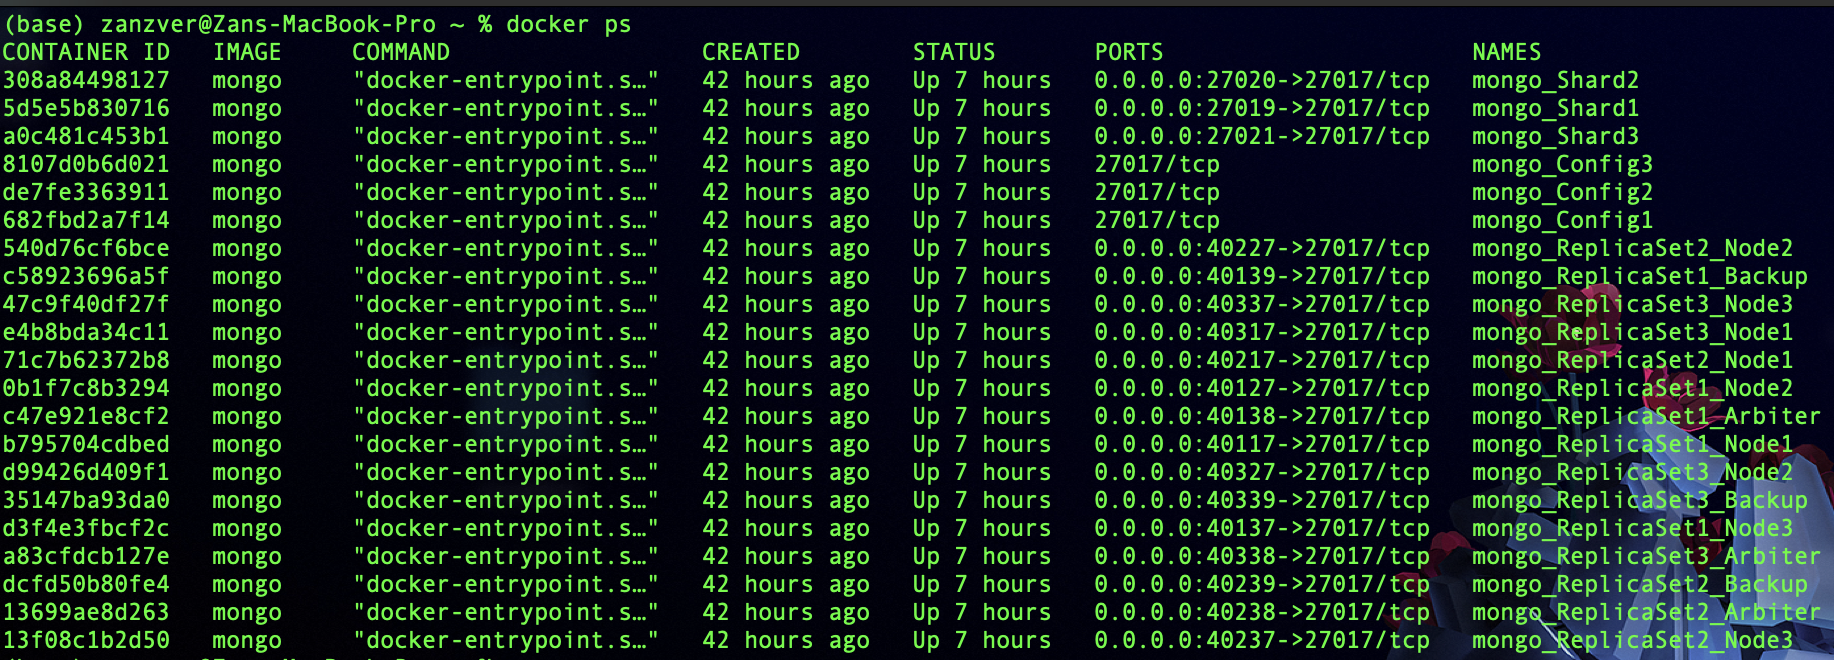
\includegraphics[scale=0.45]{img/allDockerContainers.png}
\centering
\caption{Containers displayed in terminal}
\end{figure}

\subsubsection{Step 3 - Fill the database}
To fill the database, Python scrip was used for inserting random data.
\newline
First thing is to specify how many users we want. 
\begin{lstlisting}[language=Python, caption=Call createUser function]
createUser(10)
\end{lstlisting}
Based on the input number (10 in our case) users are going to be created.
\begin{lstlisting}[language=Python, caption=Showcase of createUser function]
def createUser(num):
    for i in range(num):
        firstname = names.get_first_name()
        lastname = names.get_last_name()
        items = ["", str(random.randrange(1,999))]
        random_item = random.choice(items)
        random_email = random.choice(emailProviders)
        random_address = real_random_address()
        #print(random_item)
        mydict = {
                "Username": firstname + lastname,
                "Password": randomword(10),
                "Email": firstname + "." + lastname + random_item + random_email,
                "Name": firstname,
                "Surname": lastname,
                "Location": {
                    "Address": [
                        random_address["address1"],
                        random_address["address2"]
                    ],
                    "Postcode": random_address["postalCode"],
                    "City": random_address["state"],
                    "Country": "United States"
                }
        }
        x = colUsers.insert_one(mydict)
        createItAll(x.inserted_id)
        createHistory(x.inserted_id)
\end{lstlisting}
When we create the user, we also create devices for the user.
\begin{lstlisting}[language=Python, caption=Showcase of createItAll function]
def createItAll(UserID):
    myDict = createDevices()
    colIoT_Customer_Device.insert_one(
        { "UserID" : str(UserID),
          "smart_light": myDict["smart_light"],
          "smart_fridge": myDict["smart_fridge"],
          "smart_vacuum": myDict["smart_vacuum"]
        })
    
    dict1 = createDeviceInfo()
    try:
        dict2 = colIoT_Device_Info.find_one()
        for deviceTypes in dict1.keys():
            for manufacturer in dict1[deviceTypes].keys():
                for modelName in list(dict1[deviceTypes][manufacturer])[0].keys():
                    for serialNumber in list(dict2[deviceTypes][manufacturer])[0][modelName]["Serial_Numbers"]:
                        list(dict1[deviceTypes][manufacturer])[0][modelName]["Serial_Numbers"].append(serialNumber)
        
        oldquery = colIoT_Device_Info.find_one()
        newquery = { "$set": dict1 }
        
        colIoT_Device_Info.update_one(oldquery, newquery)
    except:
        colIoT_Device_Info.insert_one(dict1)
\end{lstlisting}
As noted in the code, history for device is also generated.
\begin{lstlisting}[language=Python, caption=Showcase of createHistory]
def createHistory(userID):
    lightHistoryGenerator = random.randrange(1,30)
    fridgeHistoryGenerator = random.randrange(1,30)
    vacuumHistoryGenerator = random.randrange(1,30)
    for i in range(lightHistoryGenerator):
        colIoT_Device_History.insert_one({str(userID): {"1": createTheSmartLight()["Device_Status"]}})
    
    for i in range(fridgeHistoryGenerator):
        colIoT_Device_History.insert_one({str(userID): {"2": createTheFridge()["Device_Status"]}})
        
    for i in range(vacuumHistoryGenerator):
        colIoT_Device_History.insert_one({str(userID): {"3": createTheVauum()["Device_Status"]}})
\end{lstlisting}

\subsubsection{Step 4 - API}
Connect the database with API
\begin{lstlisting}[language=JavaScript, caption=Showcase of Mongoose connection to database]
const mongoose = require("mongoose");

mongoose.connect('mongodb://localhost:27019,localhost:27020,localhost:27021/initialDB', {useNewUrlParser: true}, (err) => {
    if(!err){
        console.log("MongoDB Conncetion Succeeded!")
    }
    else{
        console.log("Error in DB connection: " + err)
    }
});

require("./employee.model");
require("./user.model.js");
require("./IoT_Customer_Device.model.js");
require("./IoT_Device_Info.model.js");
\end{lstlisting}

\subsubsubsection{Step 5 - Indexes}
To improve database performance, we have added indexes \parencite{web:MongoIndexes}. With this, database management system has a faster way to identify location of document in our collection. Listed bellow we can see collections and their indexes.
\begin{center}
\begin{longtable}{ |m{4cm}|m{9cm}| } 
 \hline
 Collections name & Index description \\ 
 \hline
  users &   
  \begin{itemize}
    \item Index type: regular
    \item This collection can benefit on stock index {\_}id. Any other index would not be benefitial at the moment since we are not using this collection a lot. Most of the queries are done by {\_}id.
  \end{itemize} \\
  
  \hline
  iot{\_}customer{\_}devices &  
  \begin{itemize}
    \item Index type: regular
    \item In this collection we have a custom index with the name of UserID. As name suggests, this field has the value from collection users with users ID. Comparison bellow shows that index did not save us much time but on the document examined section, we have navigated straight to our document. If this would be larger database, time would be much bigger concern.
    \item Performance without index
    \begin{itemize}
        \item executionTimeMillis : 2
        \item totalKeysExamined : 0
        \item totalDocsExamined : 1200
    \end{itemize}
    \item Performance with index
    \begin{itemize}
        \item executionTimeMillis : 3
        \item totalKeysExamined : 1
        \item totalDocsExamined : 1
    \end{itemize}
  \end{itemize} \\
  
  \hline
  iot{\_}device{\_}info &  
  \begin{itemize}
    \item Index type: regular
    \item This collection is small (at the moment) and it does not benefit much from indexing. But in case we wanted to index it, we would do it by device type and its manufacturer.
    \item Performance without index
    \begin{itemize}
        \item executionTimeMillis : 0
        \item totalKeysExamined : 0
        \item totalDocsExamined : 1
    \end{itemize}
    \item Performance with index
    \begin{itemize}
        \item executionTimeMillis : 0
        \item totalKeysExamined : 0
        \item totalDocsExamined : 1
    \end{itemize}
  \end{itemize} \\
  
  \hline
 iot{\_}device{\_}history &  
  \begin{itemize}
    \item Index type: regular
    \item History is build as UserID (key): DeviceID (value) and in the DeviceID we have history. The idea was to create a temporary index on UserID. So, when user logs in, index is created in database and when they log out, index is removed. Upon creating index, we have noticed that indexing seems to not be performing as well. In the future, we would break the UserID (key): DeviceID (value) to UserID: value of key and to DeviceID: value of device.
    \item Performance without index
    \begin{itemize}
        \item executionTimeMillis : 37
        \item totalKeysExamined : 0
        \item totalDocsExamined : 53838
    \end{itemize}
    \item Performance with index
    \begin{itemize}
        \item executionTimeMillis : 55
        \item totalKeysExamined : 53838
        \item totalDocsExamined : 53838
    \end{itemize}
  \end{itemize} \\
  \hline
\caption{Indexes on collections}
\end{longtable}
\end{center}

\begin{figure}[H]
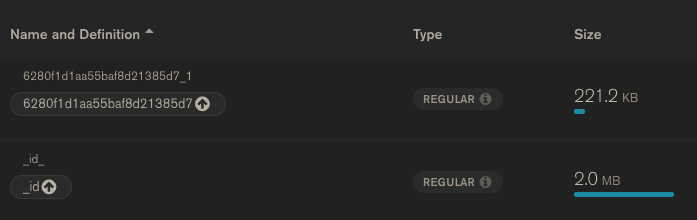
\includegraphics[scale=0.55]{img/iot_device_history-index.jpeg}
\centering
\caption{iot{\_}device{\_}history collection index}
\end{figure}


\begin{figure}[H]
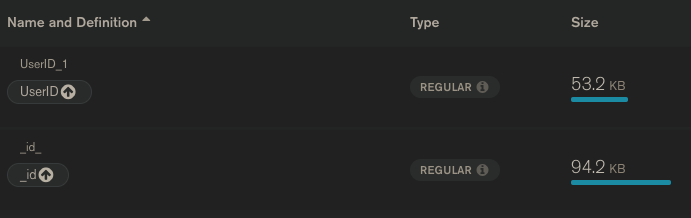
\includegraphics[scale=0.55]{img/iot_customer_devices-index.jpeg}
\centering
\caption{iot{\_}customer{\_}devices collection index}
\end{figure}


\begin{figure}[H]
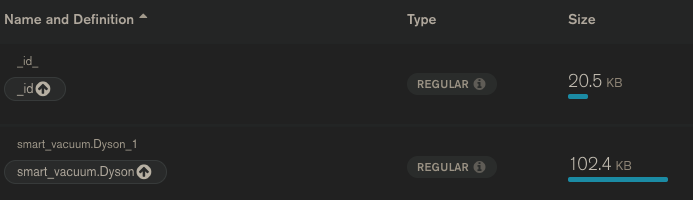
\includegraphics[scale=0.55]{img/iot_device_info-index.jpeg
}
\centering
\caption{iot{\_}device{\_}info collection index}
\end{figure}


\begin{figure}[H]
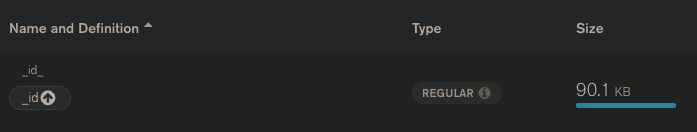
\includegraphics[scale=0.55]{img/users-index.jpeg}
\centering
\caption{users collection index}
\end{figure}

\newpage

\section{API}

\subsection{Documentation}

Design structure includes 5 main components:
\begin{itemize}
  \item home page,
  \item forgotten password,
  \item user registration,
  \item user page,
  \item admin page.
\end{itemize}
Homepage would be something simple that users and admins have in common. When admin wants to login, login section would check if user signing in is actual user or admin. With that information, the correct page would be shown.
\begin{figure}[H]
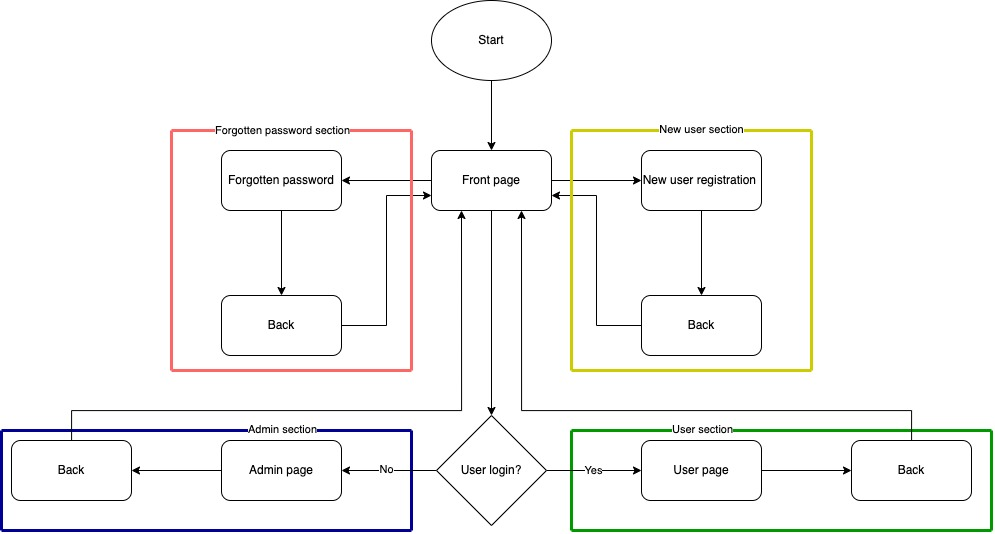
\includegraphics[scale=0.41]{img/UI-UI-simple.jpeg}
\centering
\caption{Diagram representing simple structure}
\end{figure}

Forgotten password is for users and admins to reset their passwords. Upon opening the page, user can reset the password (with inserting correct information) and be redirected to homepage. If user declines to to so, they can navigate back.
\begin{figure}[H]
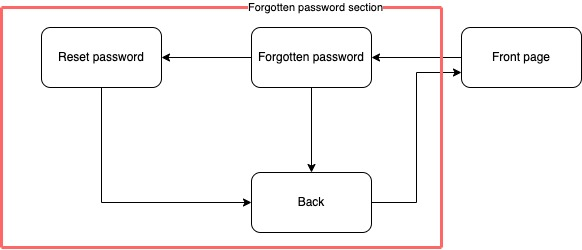
\includegraphics[scale=0.7]{img/UI-UI-forgotten-password.jpeg}
\centering
\caption{Diagram representing forgotten password}
\end{figure}

New user creation is for users to sign up for the service. On the site, user needs to fill the form in order to sign up. Once done, they are redirected to home page. If user declines to to so, they can navigate back.
\begin{figure}[H]
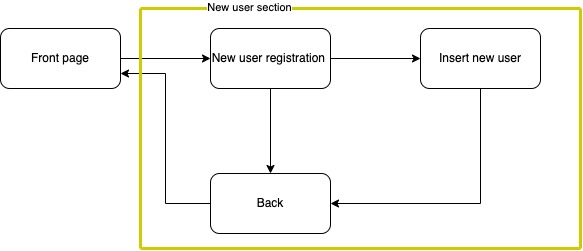
\includegraphics[scale=0.7]{img/UI-UI-new-user.jpeg}
\centering
\caption{Diagram representing new user registration}
\end{figure}

On user login, user can see how many devices he/she has per section. From there they can select section to see all devices in there. Once all devices from sections are shown, they can perform CRUD operations by adding new device, listing existing devices, adding new devices and removing existing devices.
\begin{figure}[H]
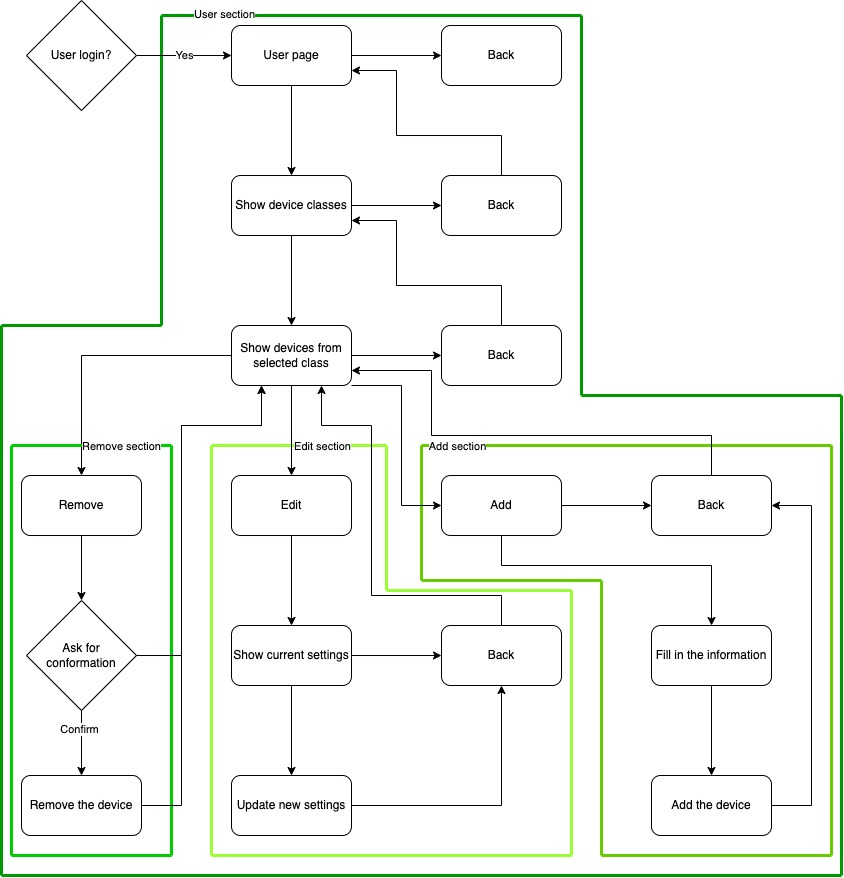
\includegraphics[scale=0.5]{img/UI-UI-users-section.jpeg}
\centering
\caption{Diagram representing user view}
\end{figure}

If user logging in is admin, he/she will be redirected to this section. In here, admin can select "show users" or "show devices" section. In case admin wants to edit user settings (promote user to admin), option is there under "show users". Another thing they can see is analysis of users (for example, usual logins). If they select "show devices", where admin can edit existing device types. Admin can also add new supported devices in "add device" section. Under device analytic, admin can see how devices are performing.
\begin{figure}[H]
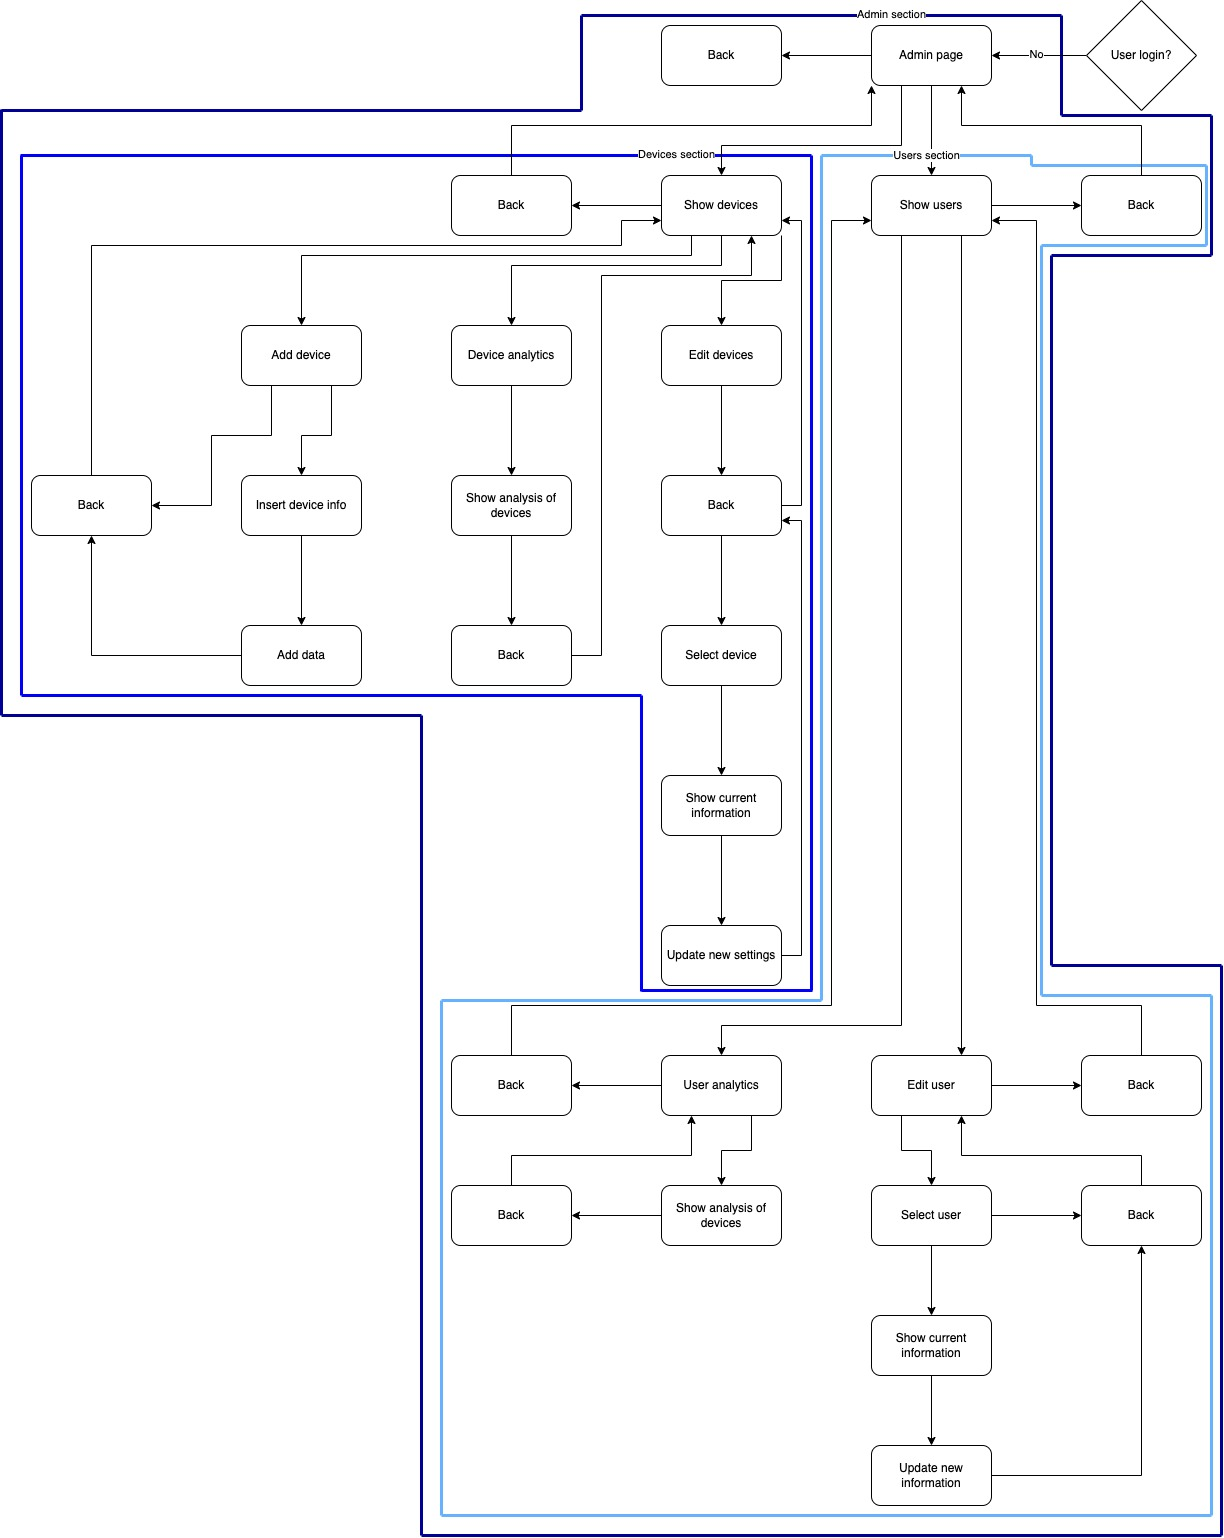
\includegraphics[scale=0.35]{img/UI-UI-admin-section.jpeg}
\centering
\caption{Diagram representing admin view}
\end{figure}

This is the same figure as on top but with all the sections expended.
\begin{figure}[H]
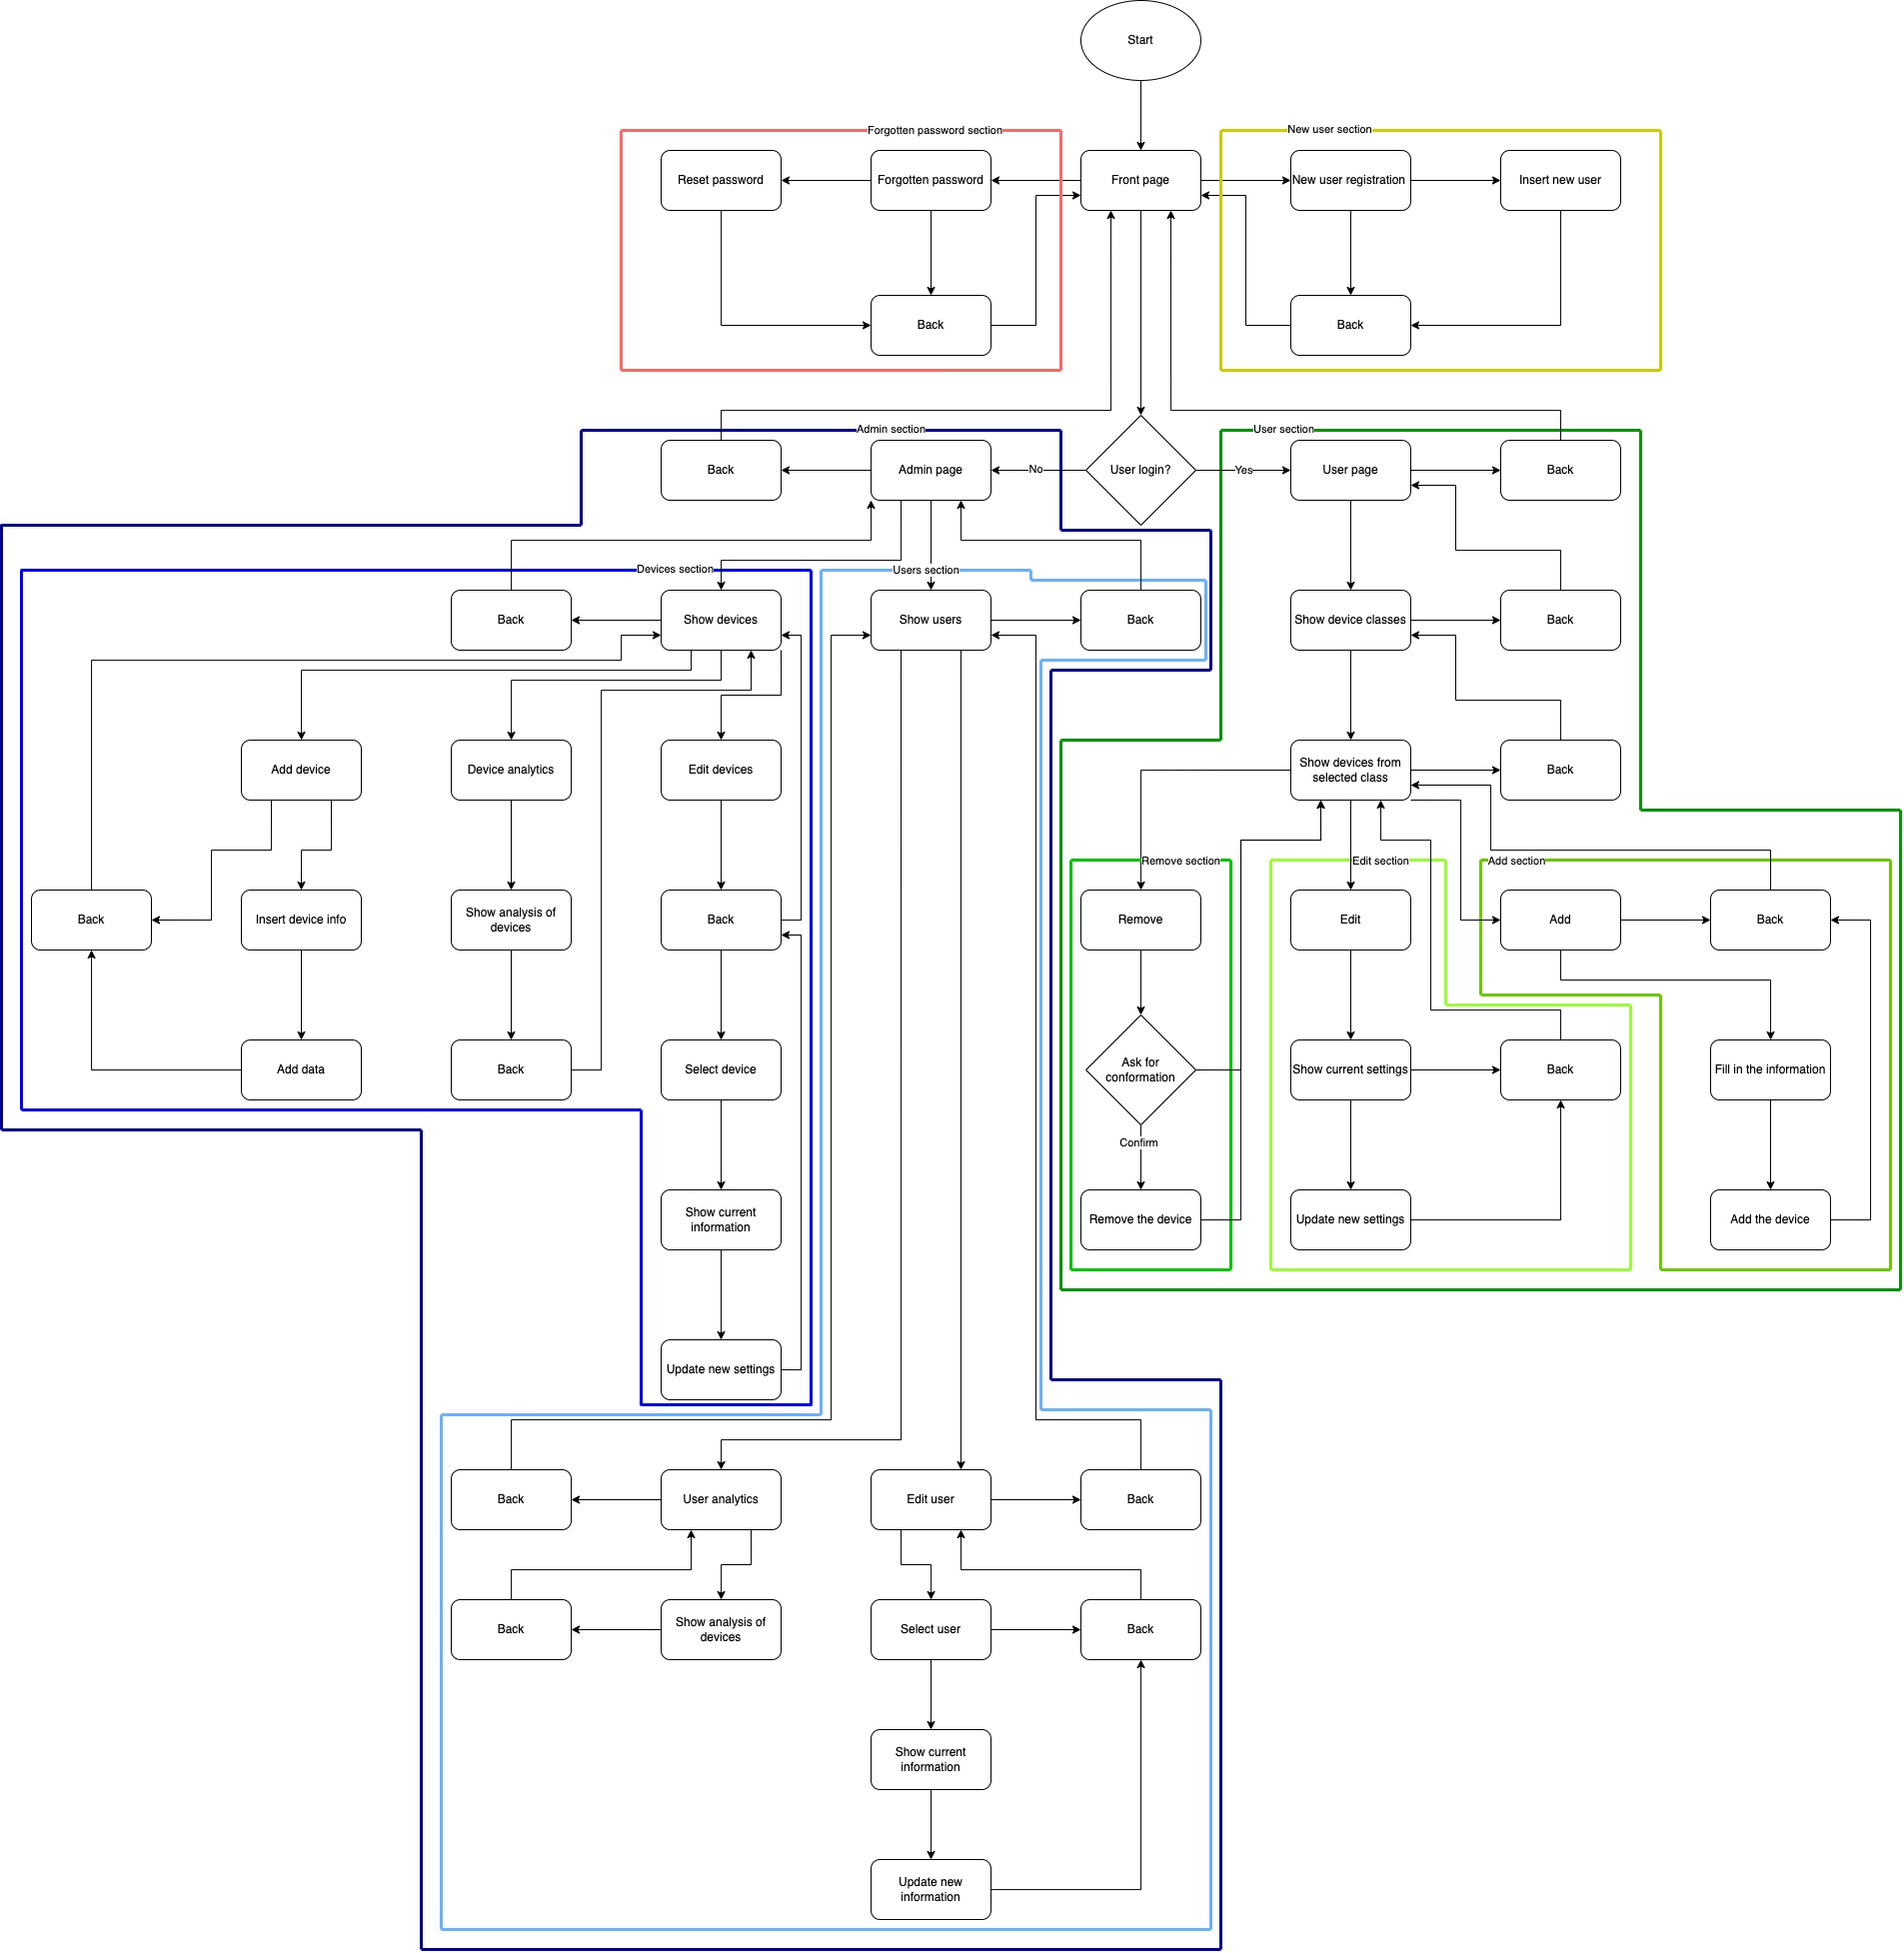
\includegraphics[scale=0.225]{img/UI-diagram.jpeg}
\centering
\caption{Detailed diagram of whole web application}
\end{figure}


\subsection{Implementation}
\subsubsection{Step 1 - Database design}
Database design was done in design section above. From there, we are implementing concepts bellow.

\subsubsection{Step 2 - Create Docker containers}
\subsubsubsection{Docker compose for nodes/replica sets}

\begin{lstlisting}[caption=Docker Compose Nodes Version]
version: '2'
services:
\end{lstlisting}

\begin{lstlisting}[caption=Docker Compose Nodes for replica set 1]
mongo_ReplicaSet1_Node1:
    container_name: mongo_ReplicaSet1_Node1
    image: mongo
    command: mongod --shardsvr --replSet mongo_ReplicaSet1 --dbpath /data/db --port 27017
    ports:
      - 40117:27017
    expose:
      - "27017"
    environment:
      TERM: xterm
    volumes:
      - mongo_ReplicaSet1_Node1:/data/db
  mongo_ReplicaSet1_Node2:
    container_name: mongo_ReplicaSet1_Node2
    image: mongo
    command: mongod --shardsvr --replSet mongo_ReplicaSet1 --dbpath /data/db --port 27017
    ports:
      - 40127:27017
    expose:
      - "27017"
    environment:
      TERM: xterm
    volumes:
      - mongo_ReplicaSet1_Node2:/data/db
  mongo_ReplicaSet1_Node3:
    container_name: mongo_ReplicaSet1_Node3
    image: mongo
    command: mongod --shardsvr --replSet mongo_ReplicaSet1 --dbpath /data/db --port 27017
    ports:
      - 40137:27017
    expose:
      - "27017"
    environment:
      TERM: xterm
    volumes:
      - mongo_ReplicaSet1_Node3:/data/db
  mongo_ReplicaSet1_Arbiter:
    container_name: mongo_ReplicaSet1_Arbiter
    image: mongo
    command: mongod --shardsvr --replSet mongo_ReplicaSet1 --dbpath /data/db --port 27017
    ports:
      - 40138:27017
    expose:
      - "27017"
    environment:
      TERM: xterm
    volumes:
      - mongo_ReplicaSet1_Arbiter:/data/db
  mongo_ReplicaSet1_Backup:
    container_name: mongo_ReplicaSet1_Backup
    image: mongo
    command: mongod --shardsvr --replSet mongo_ReplicaSet1 --dbpath /data/db --port 27017
    ports:
      - 40139:27017
    expose:
      - "27017"
    environment:
      TERM: xterm
    volumes:
      - mongo_ReplicaSet1_Backup:/data/db
\end{lstlisting}

\begin{lstlisting}[caption=Docker Compose Nodes for replica set 2]
mongo_ReplicaSet2_Node1:
    container_name: mongo_ReplicaSet2_Node1
    image: mongo
    command: mongod --shardsvr --replSet mongo_ReplicaSet2 --dbpath /data/db --port 27017
    ports:
      - 40217:27017
    expose:
      - "27017"
    environment:
      TERM: xterm
    volumes:
      - mongo_ReplicaSet2_Node1:/data/db
  mongo_ReplicaSet2_Node2:
    container_name: mongo_ReplicaSet2_Node2
    image: mongo
    command: mongod --shardsvr --replSet mongo_ReplicaSet2 --dbpath /data/db --port 27017
    ports:
      - 40227:27017
    expose:
      - "27017"
    environment:
      TERM: xterm
    volumes:
      - mongo_ReplicaSet2_Node2:/data/db
  mongo_ReplicaSet2_Node3:
    container_name: mongo_ReplicaSet2_Node3
    image: mongo
    command: mongod --shardsvr --replSet mongo_ReplicaSet2 --dbpath /data/db --port 27017
    ports:
      - 40237:27017
    expose:
      - "27017"
    environment:
      TERM: xterm
    volumes:
      - mongo_ReplicaSet2_Node3:/data/db
  mongo_ReplicaSet2_Arbiter:
    container_name: mongo_ReplicaSet2_Arbiter
    image: mongo
    command: mongod --shardsvr --replSet mongo_ReplicaSet2 --dbpath /data/db --port 27017
    ports:
      - 40238:27017
    expose:
      - "27017"
    environment:
      TERM: xterm
    volumes:
      - mongo_ReplicaSet2_Arbiter:/data/db
  mongo_ReplicaSet2_Backup:
    container_name: mongo_ReplicaSet2_Backup
    image: mongo
    command: mongod --shardsvr --replSet mongo_ReplicaSet2 --dbpath /data/db --port 27017
    ports:
      - 40239:27017
    expose:
      - "27017"
    environment:
      TERM: xterm
    volumes:
      - mongo_ReplicaSet2_Backup:/data/db
\end{lstlisting}

\begin{lstlisting}[caption=Docker Compose Nodes for replica set 3]
mongo_ReplicaSet3_Node1:
    container_name: mongo_ReplicaSet3_Node1
    image: mongo
    command: mongod --shardsvr --replSet mongo_ReplicaSet3 --dbpath /data/db --port 27017
    ports:
      - 40317:27017
    expose:
      - "27017"
    environment:
      TERM: xterm
    volumes:
      - mongo_ReplicaSet3_Node1:/data/db
  mongo_ReplicaSet3_Node2:
    container_name: mongo_ReplicaSet3_Node2
    image: mongo
    command: mongod --shardsvr --replSet mongo_ReplicaSet3 --dbpath /data/db --port 27017
    ports:
      - 40327:27017
    expose:
      - "27017"
    environment:
      TERM: xterm
    volumes:
      - mongo_ReplicaSet3_Node2:/data/db
  mongo_ReplicaSet3_Node3:
    container_name: mongo_ReplicaSet3_Node3
    image: mongo
    command: mongod --shardsvr --replSet mongo_ReplicaSet3 --dbpath /data/db --port 27017
    ports:
      - 40337:27017
    expose:
      - "27017"
    environment:
      TERM: xterm
    volumes:
      - mongo_ReplicaSet3_Node3:/data/db
  mongo_ReplicaSet3_Arbiter:
    container_name: mongo_ReplicaSet3_Arbiter
    image: mongo
    command: mongod --shardsvr --replSet mongo_ReplicaSet3 --dbpath /data/db --port 27017
    ports:
      - 40338:27017
    expose:
      - "27017"
    environment:
      TERM: xterm
    volumes:
      - mongo_ReplicaSet3_Arbiter:/data/db
  mongo_ReplicaSet3_Backup:
    container_name: mongo_ReplicaSet3_Backup
    image: mongo
    command: mongod --shardsvr --replSet mongo_ReplicaSet3 --dbpath /data/db --port 27017
    ports:
      - 40339:27017
    expose:
      - "27017"
    environment:
      TERM: xterm
    volumes:
      - mongo_ReplicaSet3_Backup:/data/db
\end{lstlisting}

\begin{lstlisting}[caption=Docker Compose storage for nodes]
volumes:
  mongo_ReplicaSet1_Node1: {}
  mongo_ReplicaSet1_Node2: {}
  mongo_ReplicaSet1_Node3: {}
  mongo_ReplicaSet1_Arbiter: {}
  mongo_ReplicaSet1_Backup: {}
  mongo_ReplicaSet2_Node1: {}
  mongo_ReplicaSet2_Node2: {}
  mongo_ReplicaSet2_Node3: {}
  mongo_ReplicaSet2_Arbiter: {}
  mongo_ReplicaSet2_Backup: {}
  mongo_ReplicaSet3_Node1: {}
  mongo_ReplicaSet3_Node2: {}
  mongo_ReplicaSet3_Node3: {}
  mongo_ReplicaSet3_Arbiter: {}
  mongo_ReplicaSet3_Backup: {}
\end{lstlisting}
\subsubsubsection{Docker compose for config servers}
\begin{lstlisting}[caption=Docker Compose Config Version]
version: '2'
services:
\end{lstlisting}

\begin{lstlisting}[caption=Docker Compose Config 1]
mongo_Config1:
      container_name: mongo_Config1
      image: mongo
      command: mongod --configsvr --replSet mongo_ReplicaSet1_Conf --dbpath /data/db --port 27017
      environment:
        TERM: xterm
      expose:
        - "27017"
      volumes:
        - mongo_Config1:/data/db
\end{lstlisting}

\begin{lstlisting}[caption=Docker Compose Config 2]
mongo_Config2:
      container_name: mongo_Config2
      image: mongo
      command: mongod --configsvr --replSet mongo_ReplicaSet1_Conf --dbpath /data/db --port 27017
      environment:
        TERM: xterm
      expose:
        - "27017"
      volumes:
        - mongo_Config2:/data/db
\end{lstlisting}

\begin{lstlisting}[caption=Docker Compose Config 3]
  mongo_Config3:
      container_name: mongo_Config3
      image: mongo
      command: mongod --configsvr --replSet mongo_ReplicaSet1_Conf --dbpath /data/db --port 27017
      environment:
        TERM: xterm
      expose:
        - "27017"
      volumes:
        - mongo_Config3:/data/db
\end{lstlisting}

\begin{lstlisting}[caption=Docker Compose storage for Config]
volumes:
  mongo_Config1: {}
  mongo_Config2: {}
  mongo_Config3: {}
\end{lstlisting}
\subsubsubsection{Docker compose for routers}
\begin{lstlisting}[caption=Docker Compose Router Version]
version: '2'
services:
\end{lstlisting}

\begin{lstlisting}[caption=Docker Compose router 1]
mongo_Shard1:
    container_name: mongo_Shard1
    image: mongo
    command: mongos --configdb mongo_ReplicaSet1_Conf/mongo_Config1:27017,mongo_Config2:27017,mongo_Config3:27017 --port 27017 --bind_ip 0.0.0.0
    ports:
      - 27019:27017
    expose:
      - "27017"
    volumes:
      - /etc/localtime:/etc/localtime:ro
\end{lstlisting}

\begin{lstlisting}[caption=Docker Compose router 2]
  mongo_Shard2:
    container_name: mongo_Shard2
    image: mongo
    command: mongos --configdb mongo_ReplicaSet1_Conf/mongo_Config1:27017,mongo_Config2:27017,mongo_Config3:27017 --port 27017 --bind_ip 0.0.0.0
    ports:
      - 27020:27017
    expose:
      - "27017"
    volumes:
      - /etc/localtime:/etc/localtime:ro
\end{lstlisting}

\begin{lstlisting}[caption=Docker Compose router 3]
  mongo_Shard3:
    container_name: mongo_Shard3
    image: mongo
    command: mongos --configdb mongo_ReplicaSet1_Conf/mongo_Config1:27017,mongo_Config2:27017,mongo_Config3:27017 --port 27017 --bind_ip 0.0.0.0
    ports:
      - 27021:27017
    expose:
      - "27017"
    volumes:
      - /etc/localtime:/etc/localtime:ro
\end{lstlisting}
\subsubsubsection{Execute docker compose}
\paragraph{Run docker compose files}\mbox{}\\
setup replica $\xrightarrow{}$ set nodes - 5 nodes per 3 replica sets $\xrightarrow{}$ 15 docker nodes are created
\begin{lstlisting}[language=Bash, caption=Create 15 Mongo nodes]
sudo docker-compose -f docker-compose.yaml up -d
\end{lstlisting}
setup config $\xrightarrow{}$ 3 config (docker) servers are running
\begin{lstlisting}[language=Bash, caption=Create config servers]
sudo docker-compose -f mongod.yaml up -d
\end{lstlisting}
setup router $\xrightarrow{}$ 3 mongos (router) dockers are running
\begin{lstlisting}[language=Bash, caption=Create router servers]
sudo docker-compose -f mongos.yaml up -d
\end{lstlisting}

%=========================================================================================================
% configure config servers replica set
%=========================================================================================================
\paragraph{Configure config servers replica set}\mbox{}\\
Replica set 1
\begin{lstlisting}[language=Bash, caption=Set config1]
docker exec -it mongo_Config1 bash -c "echo 'rs.initiate(
    {_id: \"mongo_ReplicaSet1_Conf\",configsvr: true, members: [
        { _id : 0, host : \"mongo_Config1\" },
        { _id : 1, host : \"mongo_Config2\" }, 
        { _id : 2, host : \"mongo_Config3\" }
        ]
    })
' | mongosh"
\end{lstlisting}
Replica set 2
\begin{lstlisting}[language=Bash, caption=Set config2]
docker exec -it mongo_Config2 bash -c "echo 'rs.initiate(
    {_id: \"mongo_ReplicaSet1_Conf\",configsvr: true, members: [
        { _id : 0, host : \"mongo_Config1\" },
        { _id : 1, host : \"mongo_Config2\" }, 
        { _id : 2, host : \"mongo_Config3\" }
        ]
    }
)' | mongosh"
\end{lstlisting}
Replica set 3
\begin{lstlisting}[language=Bash, caption=Set config3]
docker exec -it mongo_Config3 bash -c "echo 'rs.initiate(
    {_id: \"mongo_ReplicaSet1_Conf\",configsvr: true, members: [
        { _id : 0, host : \"mongo_Config1\" },
        { _id : 1, host : \"mongo_Config2\" }, 
        { _id : 2, host : \"mongo_Config3\" }
        ]
    }
)' | mongosh"
\end{lstlisting}

%=========================================================================================================
% check config server replica set status
%=========================================================================================================
\paragraph{Check config server replica set status}\mbox{}\\
\begin{lstlisting}[language=Bash, caption=Check replica set status]
docker exec -it mongo_Config1 bash -c "echo 'rs.status()' | mongosh"
\end{lstlisting}

%=========================================================================================================
% build shard replica set
%=========================================================================================================
\paragraph{Build shard replica set}\mbox{}\\
Replica set 1
\begin{lstlisting}[language=Bash, caption=Build replica set 1]
docker exec -it mongo_ReplicaSet1_Node1 bash -c "echo 'rs.initiate(
    {_id : \"mongo_ReplicaSet1\", members: [
        { _id : 0, host : \"mongo_ReplicaSet1_Node1\" },
        { _id : 1, host : \"mongo_ReplicaSet1_Node2\" },
        { _id : 2, host : \"mongo_ReplicaSet1_Node3\" },
        { _id : 3, host : \"mongo_ReplicaSet1_Arbiter\", arbiterOnly: true},
        { _id : 4, host : \"mongo_ReplicaSet1_Backup\", hidden: true}
        ]
    }
)' | mongosh"
\end{lstlisting}
Replica set 2
\begin{lstlisting}[language=Bash, caption=Build replica set 2]
docker exec -it mongo_ReplicaSet2_Node1 bash -c "echo 'rs.initiate(
    {_id : \"mongo_ReplicaSet2\", members: [
        { _id : 0, host : \"mongo_ReplicaSet2_Node1\" },
        { _id : 1, host : \"mongo_ReplicaSet2_Node2\" },
        { _id : 2, host : \"mongo_ReplicaSet2_Node3\" },
        { _id : 3, host : \"mongo_ReplicaSet2_Arbiter\", arbiterOnly: true},
        { _id : 4, host : \"mongo_ReplicaSet2_Backup\", hidden: true}
        ]
    }
)' | mongosh"
\end{lstlisting}
Replica set 3
\begin{lstlisting}[language=Bash, caption=Build replica set 3]
docker exec -it mongo_ReplicaSet3_Node1 bash -c "echo 'rs.initiate(
    {_id : \"mongo_ReplicaSet3\", members: [
        { _id : 0, host : \"mongo_ReplicaSet3_Node1\" },
        { _id : 1, host : \"mongo_ReplicaSet3_Node2\" },
        { _id : 2, host : \"mongo_ReplicaSet3_Node3\" },
        { _id : 3, host : \"mongo_ReplicaSet3_Arbiter\", arbiterOnly: true},
        { _id : 4, host : \"mongo_ReplicaSet3_Backup\", hidden: true}
        ]
    }
)' | mongosh"
\end{lstlisting}

%=========================================================================================================
% check status primary-secondary
%=========================================================================================================
\paragraph{Check status primary-secondary}\mbox{}\\
Status for replica set 1
\begin{lstlisting}[language=Bash, caption=Check status of replica set 1]
docker exec -it mongo_ReplicaSet1_Node1 bash -c "echo 'rs.status()' | mongosh"
\end{lstlisting}
Status for replica set 2
\begin{lstlisting}[language=Bash, caption=Check status of replica set 2]
docker exec -it mongo_ReplicaSet2_Node1 bash -c "echo 'rs.status()' | mongosh"
\end{lstlisting}
Status for replica set 3
\begin{lstlisting}[language=Bash, caption=Check status of replica set 3]
docker exec -it mongo_ReplicaSet3_Node1 bash -c "echo 'rs.status()' | mongosh"
\end{lstlisting}

%=========================================================================================================
% introduce shard to the routers
%=========================================================================================================
\paragraph{Introduce replica set to the routers}\mbox{}\\
Add mongo{\_}Shard1
\begin{lstlisting}[language=Bash, caption=Introduce replica 1]
docker exec -it mongo_Shard1 bash -c "echo 'sh.addShard(\"mongo_ReplicaSet1/mongo_ReplicaSet1_Node1\")' | mongosh"
\end{lstlisting}
Add mongo{\_}Shard2
\begin{lstlisting}[language=Bash, caption=Introduce replica 2]
docker exec -it mongo_Shard2 bash -c "echo 'sh.addShard(\"mongo_ReplicaSet2/mongo_ReplicaSet2_Node1\")' | mongosh"
\end{lstlisting}
Add mongo{\_}Shard3
\begin{lstlisting}[language=Bash, caption=Introduce replica 3]
docker exec -it mongo_Shard3 bash -c "echo 'sh.addShard(\"mongo_ReplicaSet3/mongo_ReplicaSet3_Node1\")' | mongosh"
\end{lstlisting}

%=========================================================================================================
% get shard status
%=========================================================================================================
\paragraph{Get shard status}\mbox{}\\
\begin{lstlisting}[language=Bash, caption=Get shard status]
docker exec -it mongo_Shard1 bash -c "echo 'sh.status()' | mongosh"
\end{lstlisting}

%=========================================================================================================
% create test db
%=========================================================================================================
\paragraph{Create test db}\mbox{}\\
Create test db in shard mongo{\_}ReplicaSet{\_}1 for testing.
\begin{lstlisting}[language=Bash, caption=Create test db]
docker exec -it mongo_ReplicaSet1_Node1 bash -c "echo 'use testDb' | mongosh"
\end{lstlisting}

%=========================================================================================================
% enable sharding for new db
%=========================================================================================================
\paragraph{Enable sharding for new db}\mbox{}\\
Test sharding of new database.
\begin{lstlisting}[language=Bash, caption=Enable sharding for new db]
docker exec -it mongo_Shard1 bash -c "echo 'sh.enableSharding(\"testDb\")' | mongosh"
\end{lstlisting}

%=========================================================================================================
% create test collection
%=========================================================================================================
\paragraph{Create test collection}\mbox{}\\
Create test collection for further testing.
\begin{lstlisting}[language=Bash, caption=Create test collection RS1]
docker exec -it mongo_ReplicaSet1_Node1 bash -c "echo 'db.createCollection(\"testDb.testCollection\")' | mongosh"
\end{lstlisting}
\begin{lstlisting}[language=Bash, caption=Create test collection RS2]
docker exec -it mongo_ReplicaSet2_Node1 bash -c "echo 'db.createCollection(\"testDb.testCollection\")' | mongosh"
\end{lstlisting}
\begin{lstlisting}[language=Bash, caption=Create test collection RS3]
docker exec -it mongo_ReplicaSet3_Node1 bash -c "echo 'db.createCollection(\"testDb.testCollection\")' | mongosh"
\end{lstlisting}

%=========================================================================================================
% shard based on the key
%=========================================================================================================
\paragraph{Shard based on the key}\mbox{}\\
Test sharding collection based on the key.
\begin{lstlisting}[language=Bash, caption=Shard based on the key]
docker exec -it mongo_Shard1 bash -c "echo 'sh.shardCollection(\"testDb.testCollection\", {\"shardingField\" : 1})' | mongosh"
\end{lstlisting}
\subsubsubsection{Showcase of docker containers}
At the end we have 21 docker containers that are database related. All of the Docker containers are on local network (localhost) in our case. In the table bellow, we can see the function they have.

\begin{center}
\begin{longtable}{ |m{5.5cm}|m{6cm}|m{1.5cm}| } 
 \hline
    Container name & Container description & Port \\ 
 \hline
 \hline
    mongo{\_}ReplicaSet1{\_}Node1 & Storage node 1 for replica set 1 & 40117\\ 
 \hline
    mongo{\_}ReplicaSet1{\_}Node2 & Storage node 2 for replica set 1 & 40127\\ 
 \hline
    mongo{\_}ReplicaSet1{\_}Node3 & Storage node 3 for replica set 1 & 40137\\ 
 \hline
    mongo{\_}ReplicaSet1{\_}Arbiter & Tie breaker for replica set 1 & 40147\\ 
 \hline
    mongo{\_}ReplicaSet1{\_}Backup & Backup node for replica set 1 & 40157\\ 
 \hline
 \hline
    mongo{\_}ReplicaSet2{\_}Node1 & Storage node 1 for replica set 2 & 40217\\ 
 \hline
    mongo{\_}ReplicaSet2{\_}Node2 & Container 1 for replica set 2 & 40227\\ 
 \hline
    mongo{\_}ReplicaSet2{\_}Node3 & Container 1 for replica set 2 & 40237\\ 
 \hline
    mongo{\_}ReplicaSet2{\_}Arbiter & Tie breaker for replica set 2 & 40247\\ 
 \hline
    mongo{\_}ReplicaSet2{\_}Backup & Backup node for replica set 2 & 40257\\ 
 \hline
 \hline
    mongo{\_}ReplicaSet3{\_}Node1 & Storage node 1 for replica set 3 & 40317\\ 
 \hline
    mongo{\_}ReplicaSet3{\_}Node2 & Storage node 2 for replica set 3 & 40327\\ 
 \hline
    mongo{\_}ReplicaSet3{\_}Node3 & Storage node 3 for replica set 3 & 40337\\ 
 \hline
    mongo{\_}ReplicaSet3{\_}Arbiter & Tie breaker for replica set 3 & 40347\\ 
 \hline
    mongo{\_}ReplicaSet3{\_}Backup & Backup node for replica set 3 & 40357\\ 
 \hline
 \hline
    mongo{\_}Config1 & Configuration server 1 & 27017\\ 
 \hline
    mongo{\_}Config2 & Configuration server 2 & 27017\\ 
 \hline
    mongo{\_}Config3 & Configuration server 3 & 27017\\ 
 \hline
 \hline
    mongo{\_}Shard1 & Main router & 27019\\ 
 \hline
    mongo{\_}Shard2 & Backup router 1 & 27020\\ 
 \hline
    mongo{\_}Shard3 & Backup router 2 & 27021\\ 
 \hline
\caption{Containers used described}
\end{longtable}
\end{center}

\begin{figure}[H]
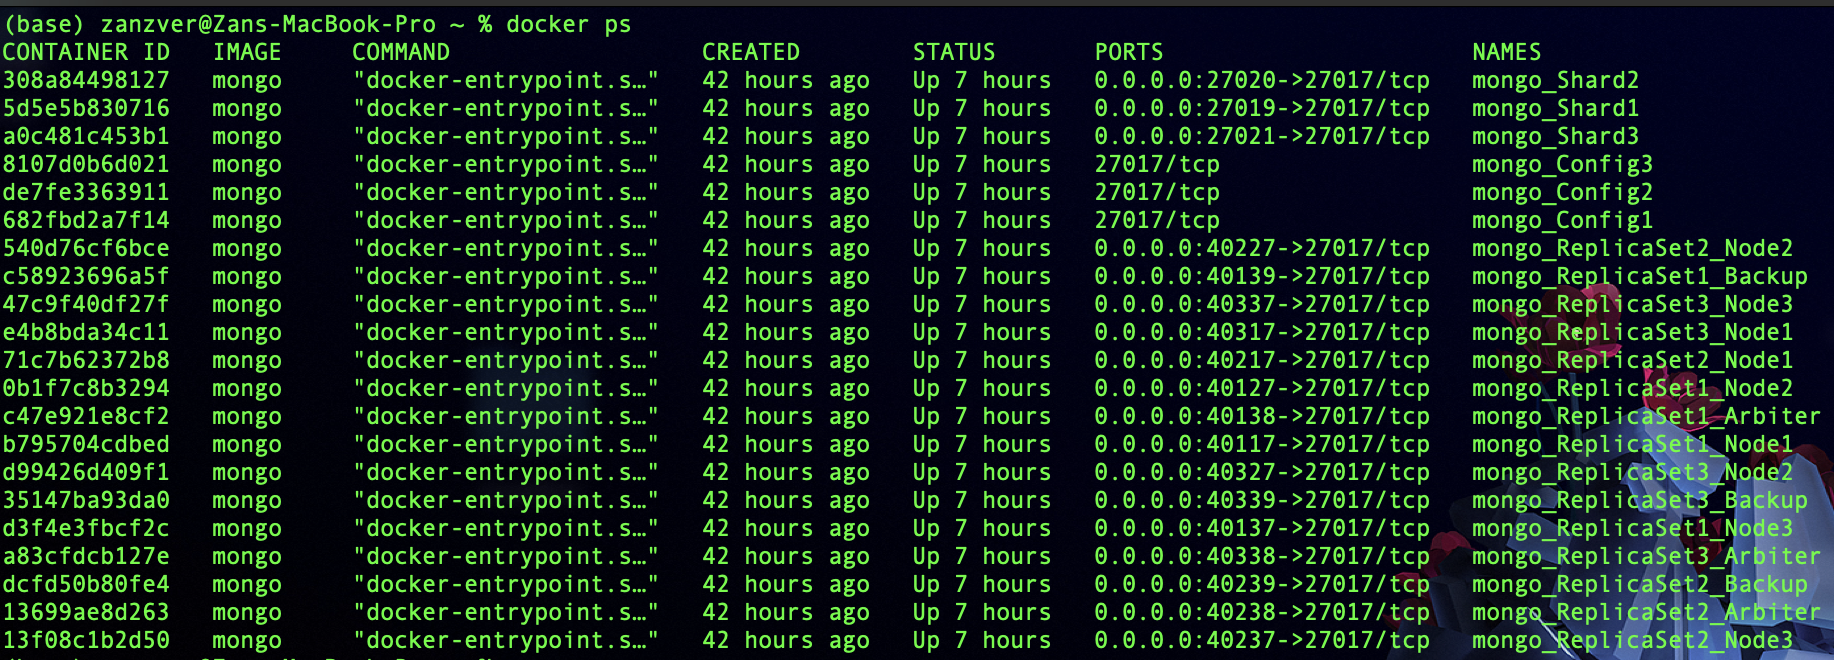
\includegraphics[scale=0.45]{img/allDockerContainers.png}
\centering
\caption{Containers displayed in terminal}
\end{figure}

\subsubsection{Step 3 - Fill the database}
To fill the database, Python scrip was used for inserting random data.
\newline
First thing is to specify how many users we want. 
\begin{lstlisting}[language=Python, caption=Call createUser function]
createUser(10)
\end{lstlisting}
Based on the input number (10 in our case) users are going to be created.
\begin{lstlisting}[language=Python, caption=Showcase of createUser function]
def createUser(num):
    for i in range(num):
        firstname = names.get_first_name()
        lastname = names.get_last_name()
        items = ["", str(random.randrange(1,999))]
        random_item = random.choice(items)
        random_email = random.choice(emailProviders)
        random_address = real_random_address()
        #print(random_item)
        mydict = {
                "Username": firstname + lastname,
                "Password": randomword(10),
                "Email": firstname + "." + lastname + random_item + random_email,
                "Name": firstname,
                "Surname": lastname,
                "Location": {
                    "Address": [
                        random_address["address1"],
                        random_address["address2"]
                    ],
                    "Postcode": random_address["postalCode"],
                    "City": random_address["state"],
                    "Country": "United States"
                }
        }
        x = colUsers.insert_one(mydict)
        createItAll(x.inserted_id)
        createHistory(x.inserted_id)
\end{lstlisting}
When we create the user, we also create devices for the user.
\begin{lstlisting}[language=Python, caption=Showcase of createItAll function]
def createItAll(UserID):
    myDict = createDevices()
    colIoT_Customer_Device.insert_one(
        { "UserID" : str(UserID),
          "smart_light": myDict["smart_light"],
          "smart_fridge": myDict["smart_fridge"],
          "smart_vacuum": myDict["smart_vacuum"]
        })
    
    dict1 = createDeviceInfo()
    try:
        dict2 = colIoT_Device_Info.find_one()
        for deviceTypes in dict1.keys():
            for manufacturer in dict1[deviceTypes].keys():
                for modelName in list(dict1[deviceTypes][manufacturer])[0].keys():
                    for serialNumber in list(dict2[deviceTypes][manufacturer])[0][modelName]["Serial_Numbers"]:
                        list(dict1[deviceTypes][manufacturer])[0][modelName]["Serial_Numbers"].append(serialNumber)
        
        oldquery = colIoT_Device_Info.find_one()
        newquery = { "$set": dict1 }
        
        colIoT_Device_Info.update_one(oldquery, newquery)
    except:
        colIoT_Device_Info.insert_one(dict1)
\end{lstlisting}
As noted in the code, history for device is also generated.
\begin{lstlisting}[language=Python, caption=Showcase of createHistory]
def createHistory(userID):
    lightHistoryGenerator = random.randrange(1,30)
    fridgeHistoryGenerator = random.randrange(1,30)
    vacuumHistoryGenerator = random.randrange(1,30)
    for i in range(lightHistoryGenerator):
        colIoT_Device_History.insert_one({str(userID): {"1": createTheSmartLight()["Device_Status"]}})
    
    for i in range(fridgeHistoryGenerator):
        colIoT_Device_History.insert_one({str(userID): {"2": createTheFridge()["Device_Status"]}})
        
    for i in range(vacuumHistoryGenerator):
        colIoT_Device_History.insert_one({str(userID): {"3": createTheVauum()["Device_Status"]}})
\end{lstlisting}

\subsubsection{Step 4 - API}
Connect the database with API
\begin{lstlisting}[language=JavaScript, caption=Showcase of Mongoose connection to database]
const mongoose = require("mongoose");

mongoose.connect('mongodb://localhost:27019,localhost:27020,localhost:27021/initialDB', {useNewUrlParser: true}, (err) => {
    if(!err){
        console.log("MongoDB Conncetion Succeeded!")
    }
    else{
        console.log("Error in DB connection: " + err)
    }
});

require("./employee.model");
require("./user.model.js");
require("./IoT_Customer_Device.model.js");
require("./IoT_Device_Info.model.js");
\end{lstlisting}

\subsubsubsection{Step 5 - Indexes}
To improve database performance, we have added indexes \parencite{web:MongoIndexes}. With this, database management system has a faster way to identify location of document in our collection. Listed bellow we can see collections and their indexes.
\begin{center}
\begin{longtable}{ |m{4cm}|m{9cm}| } 
 \hline
 Collections name & Index description \\ 
 \hline
  users &   
  \begin{itemize}
    \item Index type: regular
    \item This collection can benefit on stock index {\_}id. Any other index would not be benefitial at the moment since we are not using this collection a lot. Most of the queries are done by {\_}id.
  \end{itemize} \\
  
  \hline
  iot{\_}customer{\_}devices &  
  \begin{itemize}
    \item Index type: regular
    \item In this collection we have a custom index with the name of UserID. As name suggests, this field has the value from collection users with users ID. Comparison bellow shows that index did not save us much time but on the document examined section, we have navigated straight to our document. If this would be larger database, time would be much bigger concern.
    \item Performance without index
    \begin{itemize}
        \item executionTimeMillis : 2
        \item totalKeysExamined : 0
        \item totalDocsExamined : 1200
    \end{itemize}
    \item Performance with index
    \begin{itemize}
        \item executionTimeMillis : 3
        \item totalKeysExamined : 1
        \item totalDocsExamined : 1
    \end{itemize}
  \end{itemize} \\
  
  \hline
  iot{\_}device{\_}info &  
  \begin{itemize}
    \item Index type: regular
    \item This collection is small (at the moment) and it does not benefit much from indexing. But in case we wanted to index it, we would do it by device type and its manufacturer.
    \item Performance without index
    \begin{itemize}
        \item executionTimeMillis : 0
        \item totalKeysExamined : 0
        \item totalDocsExamined : 1
    \end{itemize}
    \item Performance with index
    \begin{itemize}
        \item executionTimeMillis : 0
        \item totalKeysExamined : 0
        \item totalDocsExamined : 1
    \end{itemize}
  \end{itemize} \\
  
  \hline
 iot{\_}device{\_}history &  
  \begin{itemize}
    \item Index type: regular
    \item History is build as UserID (key): DeviceID (value) and in the DeviceID we have history. The idea was to create a temporary index on UserID. So, when user logs in, index is created in database and when they log out, index is removed. Upon creating index, we have noticed that indexing seems to not be performing as well. In the future, we would break the UserID (key): DeviceID (value) to UserID: value of key and to DeviceID: value of device.
    \item Performance without index
    \begin{itemize}
        \item executionTimeMillis : 37
        \item totalKeysExamined : 0
        \item totalDocsExamined : 53838
    \end{itemize}
    \item Performance with index
    \begin{itemize}
        \item executionTimeMillis : 55
        \item totalKeysExamined : 53838
        \item totalDocsExamined : 53838
    \end{itemize}
  \end{itemize} \\
  \hline
\caption{Indexes on collections}
\end{longtable}
\end{center}

\begin{figure}[H]
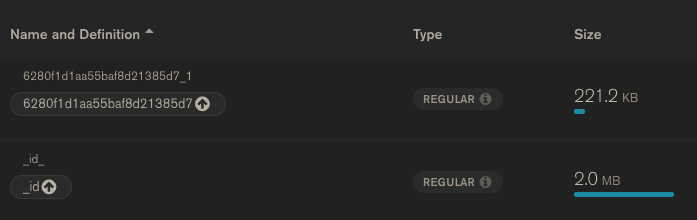
\includegraphics[scale=0.55]{img/iot_device_history-index.jpeg}
\centering
\caption{iot{\_}device{\_}history collection index}
\end{figure}


\begin{figure}[H]
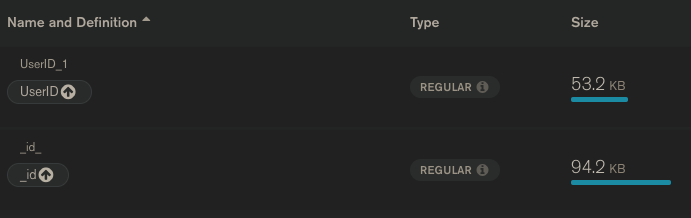
\includegraphics[scale=0.55]{img/iot_customer_devices-index.jpeg}
\centering
\caption{iot{\_}customer{\_}devices collection index}
\end{figure}


\begin{figure}[H]
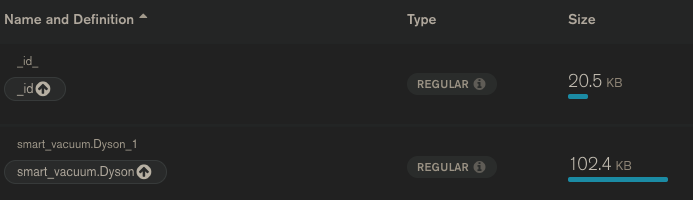
\includegraphics[scale=0.55]{img/iot_device_info-index.jpeg
}
\centering
\caption{iot{\_}device{\_}info collection index}
\end{figure}


\begin{figure}[H]
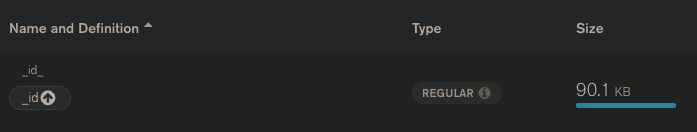
\includegraphics[scale=0.55]{img/users-index.jpeg}
\centering
\caption{users collection index}
\end{figure}
 
\newpage

\section{Summary and conclusion}
At the end, we have successfully produced a demo unit that could be implemented and scaled. On top of that, it is modular.

The database structure can scale as needed. For the company that is starting up, it wold make sense from financial standpoint to just use 1 shard instead of 3 that we have implemented. That is the great thing about NoSQL, it is simple to scale vertically or horizontally! This is specially possible with Docker. We can deploy, start/stop containers as we need.

User interface is modular as well. For our use, we have implemented NodeJS with combination of express, handlebars and mongoose. But since JavaScript is popular, this can be replaced with anything else! At the end of the day, we could use Flask (Python) with Bootstrap.
\newline
\newline
At the moment, there are still improvements that can be made. The improvements are more from technical side and range from "nice to have" to "necessary" ones. List of improvements can be found under appendix A2-improvements.
\newpage

\section{Appendixes}

\subsection{Data centers}
In the industry, the big companies have their own data centers or they are renting them from other companies like Amazon and their AWS \parencite{villamizar2016infrastructure}.
\subsubsection{Data centers across the globe}
Once you put data request across any of the websites, data is usually "piped" from your router, to ISP you have which connects you to the data center that requests is allocated for. This means, data needs to travel geographically which can take longer if it is across the globe \parencite{benson2010understanding}. 
To increase speed, companies are deploying data centers across the globe. If our application would be used worldwide, we would need to split our database. This can be done with "sharding". Lets assume the application originated in UK and that resulted in us having data in one DB already - UK shard. After some data analysis, we see that some of our customers are originating from US. To increase the speed for them, we build another shard - US shard. Later on we discover that Asian markets are joining in as well. This can lead to creation of third shard - Singapore shard.
Now we can observe the shard activity. If one shard becomes more active than the others, we can scale just one shard, or opposite, we can remove shard if it becomes financially unnecessary \parencite{alizadeh2010data}.


\subsubsection{Data rules}
As mentioned in the subsection above, one of the data centers is in the UK. Since UK is no longer a part of EU, GDPR \parencite{truong2019gdpr} is not effective on UK, but there are some other data protections placed by UK government that we would need to follow. In case our data would be in EU, we would need to respect GDPR policies in place.
Mentioned above is also Asian market. Country with the biggest population there is China but, we decided against putting shard there. The reason is "the great firewall of China". Chinese data policies are strict in sense of their government having access to all of the data. Due to privacy and anonymity, it is a better decision to have data center close to China but not in the country. This is the reason why third shard is in Singapore and not China \parencite{clayton2006ignoring}.

 \subsection{Improvements}
  Here is the list of improvements that would be useful in the application. Node that improvements are not listed in any particular order. If application would go into production, some of them could not be ignored (example: HTTPS).
  
\begin{itemize}
  \item NodeJS to docker
  \begin{itemize}
    \item at the moment, web server is running in terminal. It would be better to have docker config for it as we do have for database. With this, it is much simpler to "move" the project
  \end{itemize}
  
  \item TLS/SLL connection
  \begin{itemize}
    \item connection to the database is not secure. To improve that, we would implement TLS/SSL.
  \end{itemize}
  
  \item MongoDB LDAP user connection
  \begin{itemize}
    \item At the moment, only specified users can connect to our cluster with MongoDB. If this would be used in real world, we wold need to monitor connections from inside of the company. With LDAP, we can simply assign roles to users as permissions are needed. Root user shall not be used.
  \end{itemize}

  \item HTTPS with reverse proxy
  \begin{itemize}
    \item If this application would be on public domain, HTTPS would be crucial for this since it encrypts the connection. Also, if this would be self hosted with the company, we would need to set up some network rules and reverse proxy is one of them. One of the industry best options would be to use CloudFlare in front to defend application against DDOS attacks or any other bots \parencite{web:Cloudflare}.  
  \end{itemize}
  
  \item 2FA
  \begin{itemize}
    \item 2 factor authentication is a must now days for security. This is something our application should have in production.
  \end{itemize}
  
  \item encrypt data
  \begin{itemize}
    \item Now days, security breaches are all over the world. To combat this, we would encrypt our data so hackers cannot see what we have stored.
  \end{itemize}
  
  \item DevOPS
  \begin{itemize}
    \item In a team, having DevOPS pipeline would improve the delivery of the code. For example, fronted and backend could work on one task independently and when it comes to code merge, it would be possible due to DevOPS and its day-to-day testing \parencite{web:MSDevOPS}.
  \end{itemize}
  
  \item Improved frontend
  \begin{itemize}
    \item At the moment, NodeJS application is just for demonstration purposes. It is simple but it needs improvement and some optimisation.
  \end{itemize}
  
  \item Logging
  \begin{itemize}
    \item Servers do not send any logs back in case that anything would fail. We could use 3rd party applications like Graylog and/or Grphana to produce and visualise logs from database.
  \end{itemize}
  
  \item Analytics
  \begin{itemize}
    \item In this version, no user analytics is being produced. Database is capable of producing it, but it was not implemented. Example of analytics that we can have: number of users, most common device, etc...
  \end{itemize}
\end{itemize}


\section{References} %7
\printbibliography

\end{document}